\section{Calcuration {\em type expression}}
We described how to express type in chapter \ref{type_e001}.
In this chapter, we'll think about how to calcurate
{\em type expression} from declaration of C language.

First, we'll start to think about bellow declaration, specifically.
\begin{verbatim}
int f(double (*)(void));
\end{verbatim}
Figure \ref{decl_e001} shows syntax tree of this declaration.
\begin{figure}[htbp]
\begin{center}
%%\begin{htmlonly}
%%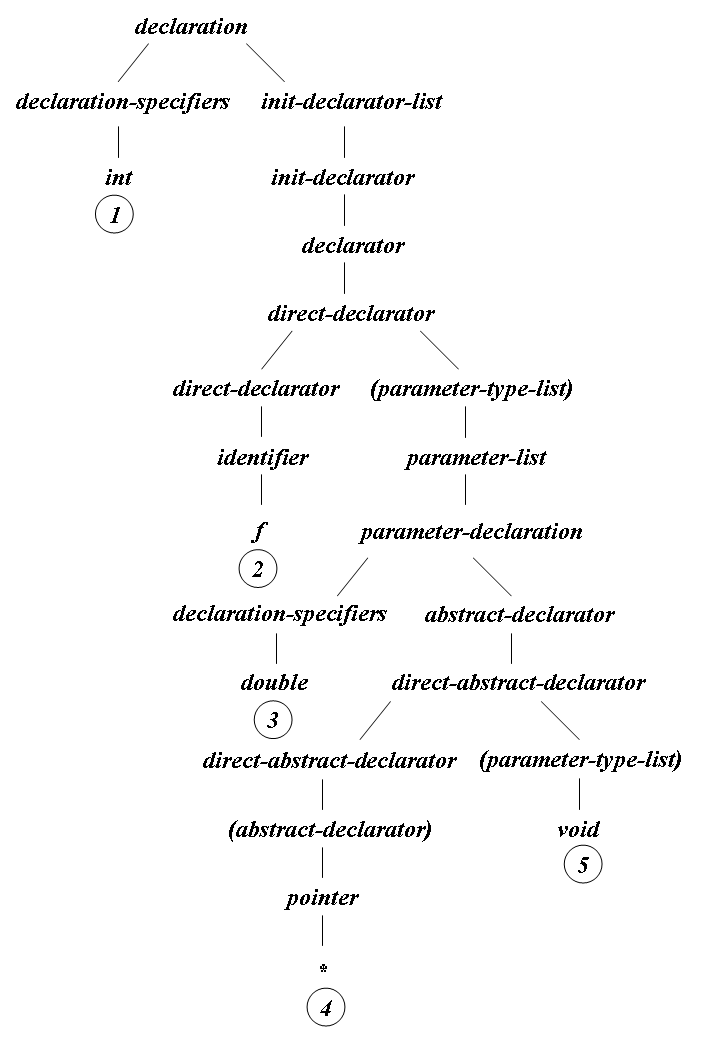
\includegraphics[width=1.0125\linewidth,height=1.4175\linewidth]{decl001.png}
%%\end{htmlonly}
%%\begin{latexonly}
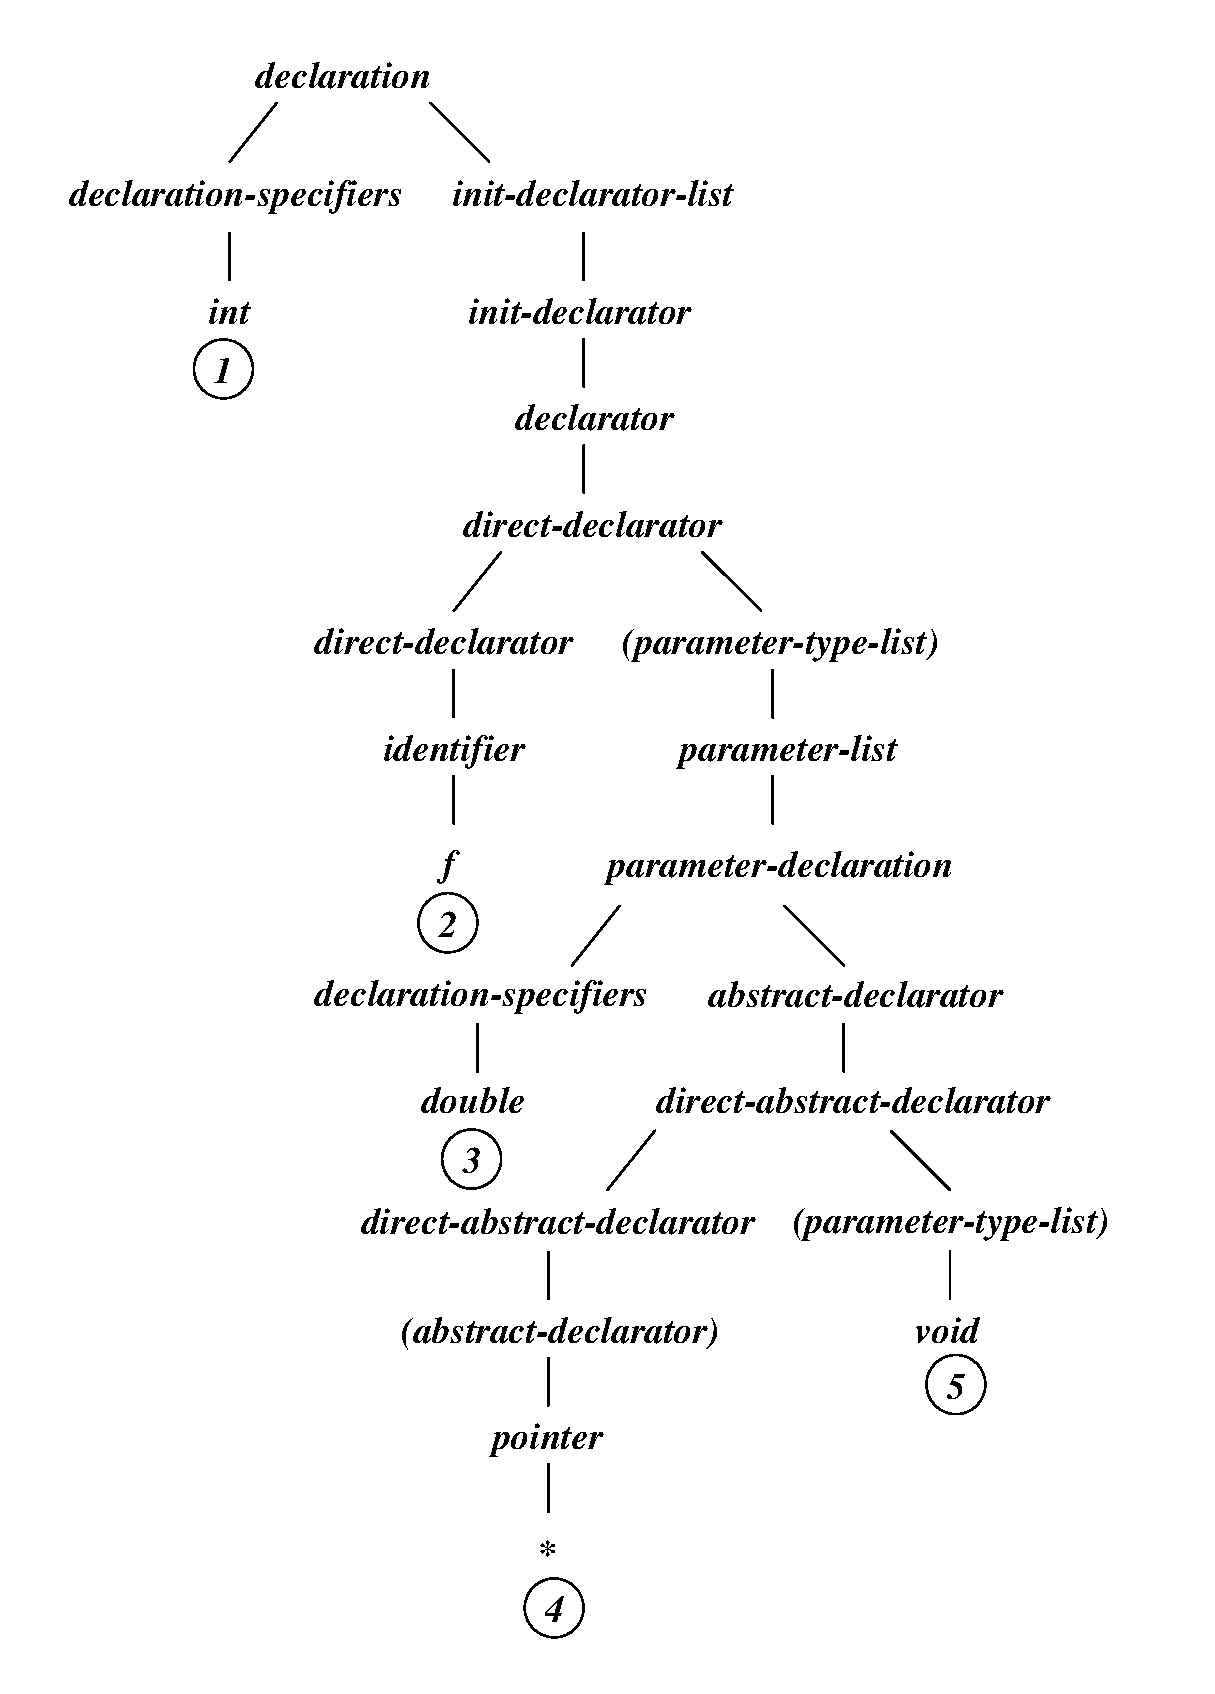
\includegraphics[width=1.0125\linewidth,height=1.4175\linewidth]{decl001.eps}
%%\end{latexonly}
\caption{syntax tree of {\tt{int f(double (*)(void));}}}
\label{decl_e001}
\end{center}
\end{figure}
Circled numbers in figure \ref{decl_e001} are reducing order
while bottom-up parsing. Frontend adds the entry according to `{\tt{f}}'
for this declaration, and the type attribute of this entry becomes
like figurue \ref{decl_e002}

\begin{figure}[htbp]
\begin{center}
%%\begin{htmlonly}
%%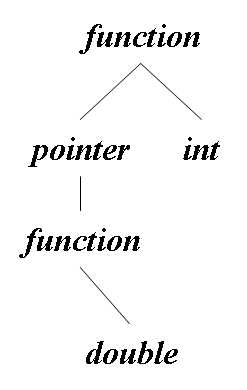
\includegraphics[width=0.5\linewidth,height=0.6\linewidth]{decl002.png}
o%%\end{htmlonly} 
%%\begin{latexonly}
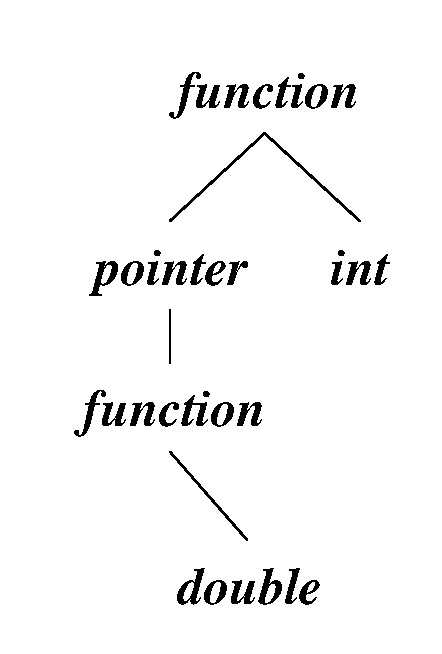
\includegraphics[width=0.5\linewidth,height=0.6\linewidth]{decl002.eps}
%%\end{latexonly}
\caption{{\em type expression} of {\tt{int f(double (*)(void));}}}
\label{decl_e002}
\end{center}
\end{figure}

Please note that when grammer symbol {\tt{pointer}} is reduced, frontend 
must create {\em type expression} ``pointer to $x$'',
and later, frontend must replace $x$ to {\em type expression} 
``function returing {\tt{double}} whick does not take argument''.

The reason of later replacing is that
grammer symbol {\tt{pointer}} is reduced
 (${\MARU{\tt 4}}$ on figure \ref{decl_e001})
and then {\tt{void}} or grammer symbol {\tt{parameter-type-list}} 
is reduced(${\MARU{\tt 5}}$ on figure \ref{decl_e001}).

Second, we'll think about bellow declaration, specifically.
\begin{verbatim}
int (*a[])();
\end{verbatim}
Figure \ref{decl_e003} shows syntax tree of this declaration
and circled numbers in figure \ref{decl_e003} are reducing order
while bottom-up parsing, samely.
\begin{figure}[htbp]
\begin{center}
%%\begin{htmlonly}
%%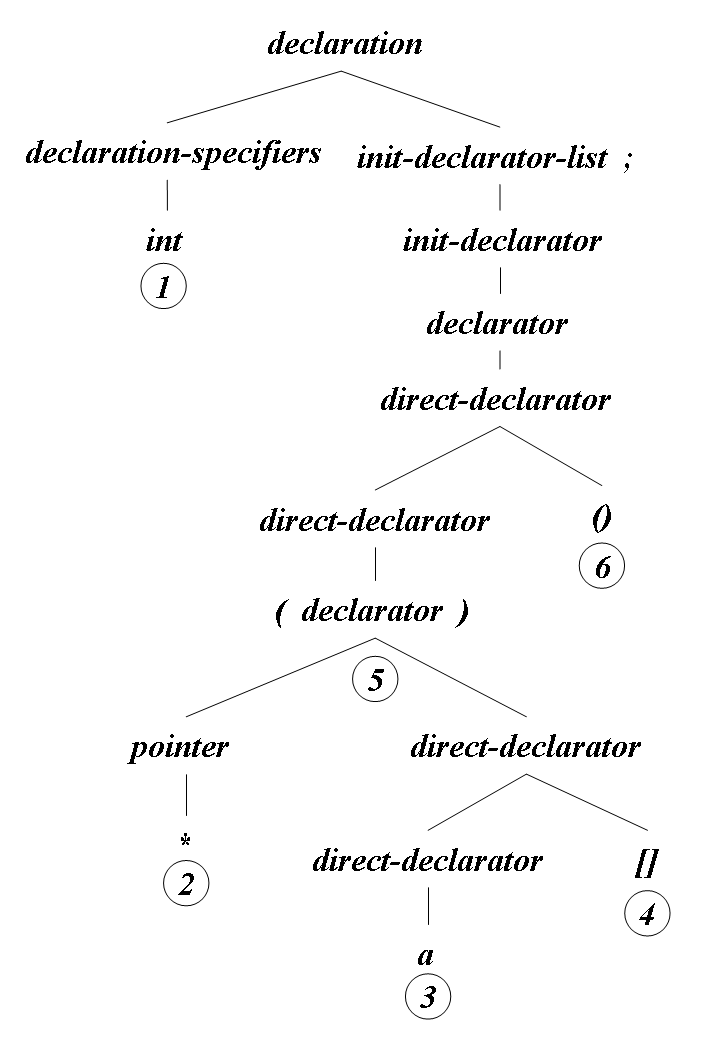
\includegraphics[width=1.0125\linewidth,height=1.4175\linewidth]{decl003.png}
%%\end{htmlonly} 
%%\begin{latexonly}
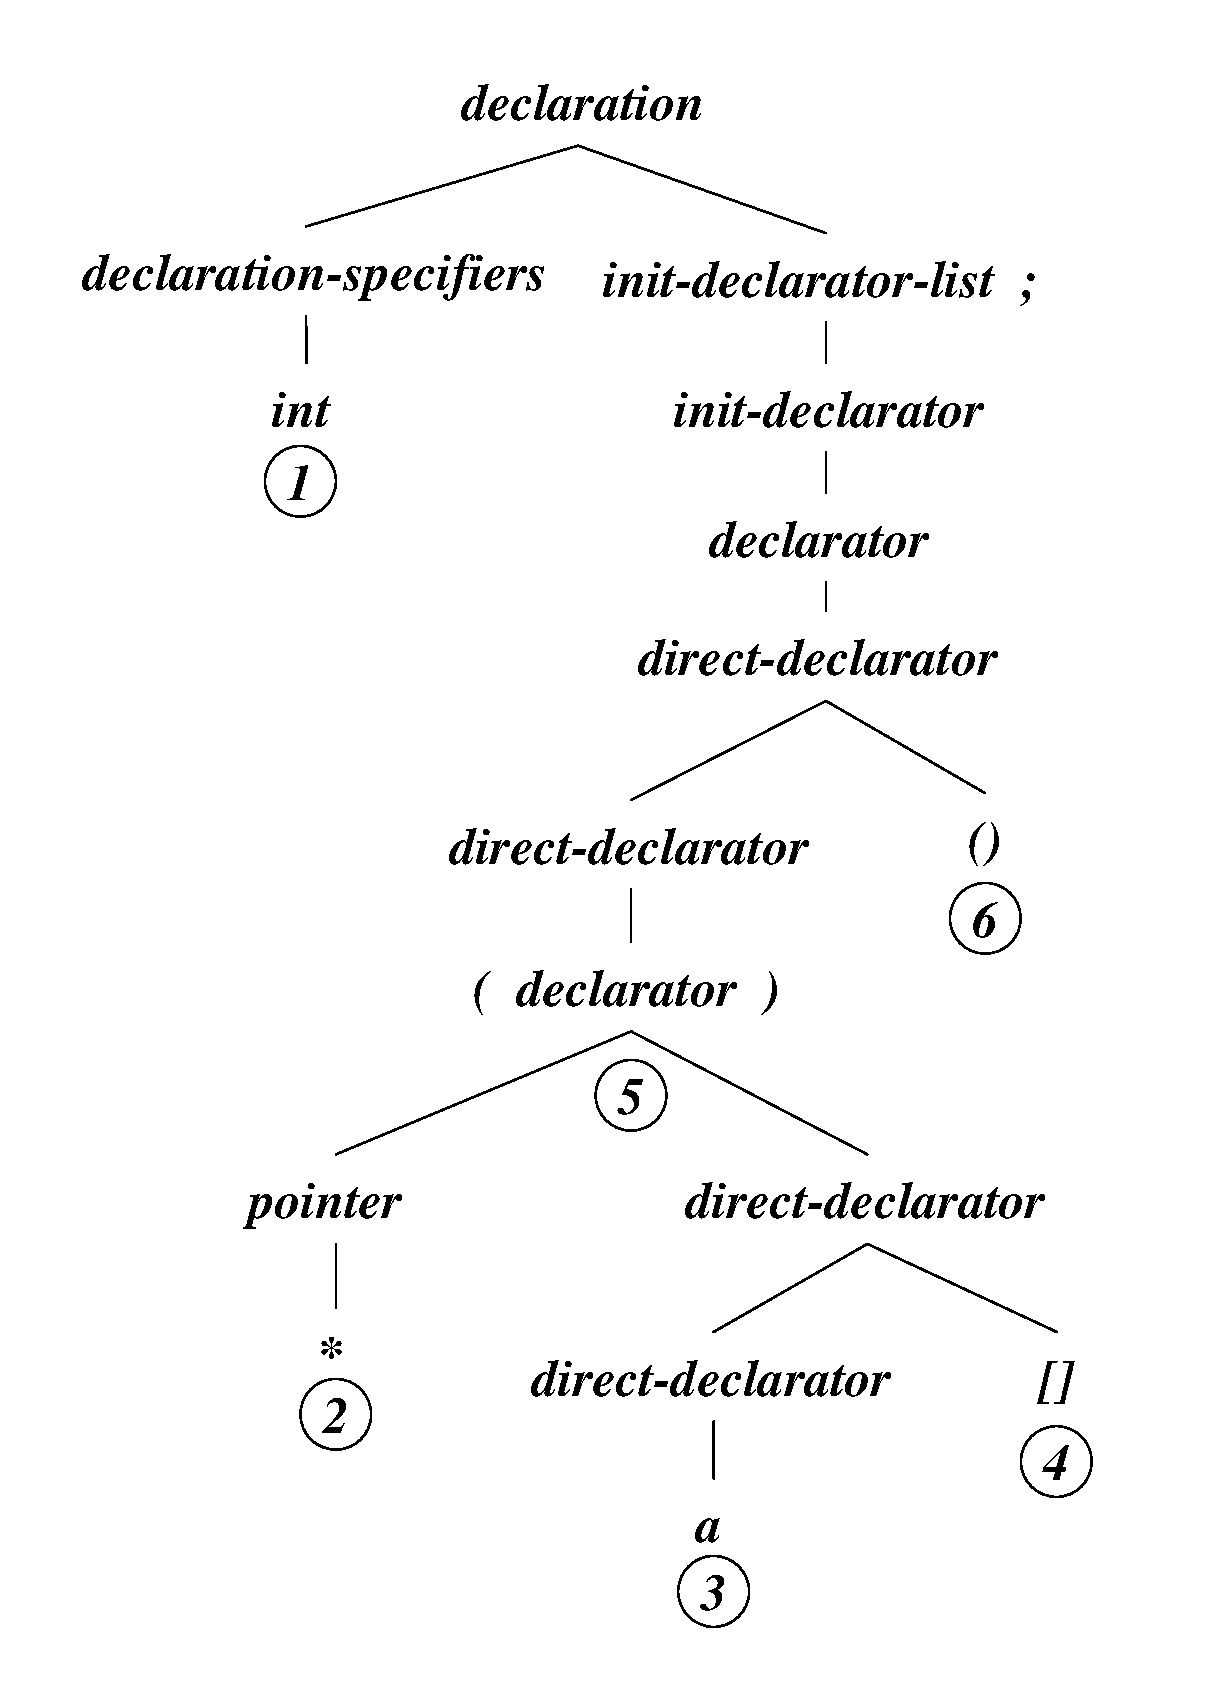
\includegraphics[width=1.0125\linewidth,height=1.4175\linewidth]{decl003.eps}
%%\end{latexonly}
\caption{syntax tree of {tt{int (*a[])()}}}
\label{decl_e003}
\end{center}
\end{figure}
 Frontend adds the entry according to `{\tt{a}}'
for this declaration, and the type attribute of this entry becomes
like figurue \ref{decl_e004}
\begin{figure}[htbp]
\begin{center}
%%\begin{htmlonly}
%%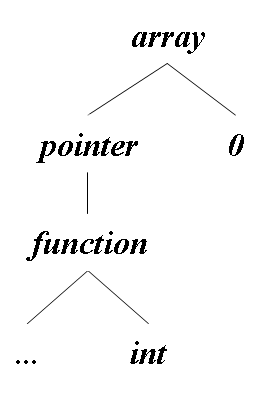
\includegraphics[width=0.5\linewidth,height=0.6\linewidth]{decl004.png}
%%\end{htmlonly} 
%%\begin{latexonly}
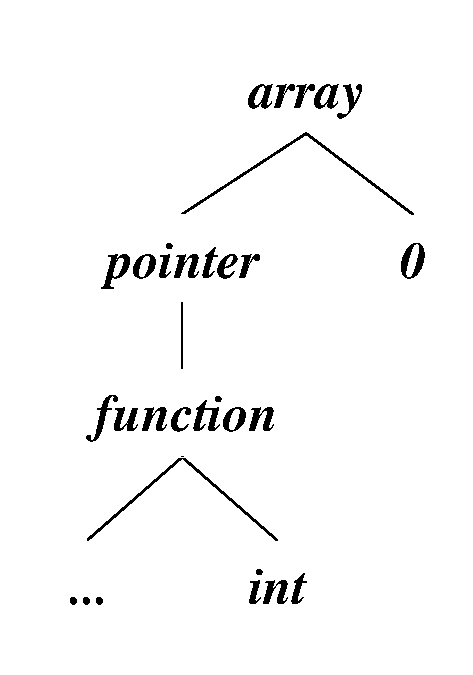
\includegraphics[width=0.5\linewidth,height=0.6\linewidth]{decl004.eps}
%%\end{latexonly}
\caption{{\em type expression} of {\tt{int (*a[])();}}}
\label{decl_e004}
\end{center}
\end{figure}

At ${\MARU{\tt 5}}$ on figure \ref{decl_e003}
\begin{verbatim}
declarator : pointer direct-declarator
\end{verbatim}
Above grammer is reduced. In this point, frontned calcurates
the type attribute of {\tt{declarator}} like bellow:

The type attribute of grammer symbol {\tt{pointer}} 
is ``pointer to $x$'', and that of grammer symbol
{\tt{direct-declarator}} is ``array of $y$''.
Now, $y$ is replaced to ``point to $x$'',
then, that of {\tt{declarator}} becomes
``array of pointer to $x$''.

And more, at ${\MARU{\tt 6}}$ on figure \ref{decl_e003}
\begin{verbatim}
direct-declarator : direct-declarator ()
\end{verbatim}
Above grammer is reduced. In this point, frontned calcurates
the type attribute of {\tt{direct-declarator}} like bellow:

The type attribute of right hand grammer symbol {\tt{direct-declarator}}
is ``array of pointer to $x$''.
Now, $x$ is replaced to ``function returing $z$'',
then, that of {\tt{direct-declarator}} becomes
``array of pointer to function returning $z$''.

Here, please remeber that if bellow grammer
\begin{verbatim}
direct-declarator : direct-declarator [ ]
\end{verbatim}
is reduced, the type attribute of left hand doesn't always become
array. And samely, if bellow grammer
\begin{verbatim}
direct-declarator : direct-declarator ( )
\end{verbatim}
is reduced, the type attribute of left hand doesn't always become
function.
Bellow declarations
\begin{verbatim}
int f()[];
int a[]();
\end{verbatim}
are error in C language, but we'll show how to calcurate
{\em type expression}. 

\begin{tabular}{cccccl}
           & {\tt{f}} &           &           &    &
                 type of {\tt{f}} is $x$                       \\
           & {\tt{f}} & {\tt{()}} &           &    &
                 type of {\tt{f}} is ``function returing $x$'' \\
           & {\tt{f}} & {\tt{()}} & {\tt{[]}} &    &
                 type of {\tt{f}} is ``function returning array of $x$'' \\
{\tt{int}} & {\tt{f}} & {\tt{()}} & {\tt{[]}} &    &
            type of {\tt{f}} is ``function returning array of {\tt{int}}'' \\
           &          &           &           &    &
                                                         \\
           & {\tt{a}} &           &           &    &
                 type of {\tt{a}} is $x$                       \\
           & {\tt{a}} & {\tt{[]}} &           &    &
                 type of {\tt{a}} is ``array of $x$'' \\
           & {\tt{a}} & {\tt{[]}} & {\tt{()}} &    &
            type of {\tt{a}} is ``array of function returing $x$'' \\
{\tt{int}} & {\tt{a}} & {\tt{[]}} & {\tt{()}} &    &
            type of {\tt{a}} is ``array of function returing {\tt{int}}'' \\
\end{tabular}

\begin{QandA}
When calcurating type expression from C language declaration,
type $x$ is replaced to type $y$. But is it necessary in different sense to
replace
some type to another type for calcurating type expression
from bellow declarations?

\begin{verbatim}
typedef int A[10];
const A a;  /* incorrect : const(array(int,10)) */
            /* correct : array(const(int),10) */

typedef int* pi;
const pi cpi;  /* correct : const(pointer(int)) */
               /* incorrect : pointer(const(int)) */
\end{verbatim}

Answer : Yes. In the different sense, it is necesssary
to replace because type qualifier
 {\tt{const}}, {\tt{volatile}}, {\tt{restrict}}
cannot qualify array or function type.
\end{QandA}

\section{Initializer}
\label{decl_e005}
Initializer is a part of declaration.
Not only it specifies the values of declared variable, but also
decides the type if declared variable has incomplete array type.
For example,
\begin{verbatim}
int a;
...
{
  int a[] = { sizeof a };  /* error : a[0] is not sizoef(int) */

  int b[] = { 0, 1, 2 };  /* int b[3]  */
}
\end{verbatim}
As described in \ref{lex_yacc_e004},
when compiler detects the minimum unit of declaration,
compiler must insert it into symbol table.

In this section, we'll think about the way to recognize
initializer. The following infomation is updated
while recognizing initializer.
\begin{itemize}
\item Initialized object type $T$
\item Set of initial value $V$, whose element is pair of offset and value.
\item Offset and max value of it $({\delta},{\delta}_{\tt{max}})$
\item The order and max value of it $(n,n_{\tt{max}})$.
      $n$ means the order in {\tt{initializer-list}} for initialized
      object type $T$.
\item The order and length of {\tt{initializer-list}} $(m,M)$.
      $m$ doesn't depend on initialized object type $T$,
      $m$ just means the position
      at {\tt{initializer-list}}. 
\end{itemize}
This infomation is denoted like bellow pair
\[
I \equiv (T,V,({\delta},{\delta}_{\tt{max}}),(n,n_{\tt{max}}),(m,M)) 
\]
And if we want to refer about $\delta_{\max}$ of $I$, we'll
use  $I.\delta_{\max}$ notation.

\begin{quotation}
{\bf Algorithm for initializer}
\begin{description}
When the token {\tt{=}} which is followed by
grammer symbol {\tt{initializer}} is reduced,
apply bellow {\bf procedure for initializer} for
\[
I \equiv (T,V,(0,0),(-1,-1),(-1,-1))
\]
where, $T$ is the type of initialized variable
which is specified {\tt{= initializer}}.
$V$ is empty set. And $-1$ denotes that
frontend doesn't work for {\tt{initializer-list}}.

\item[procedure for initializer]

\

If {\tt{initializer}} is reduced from {\tt{assignmet-expression}},
apply {\bf procedure for assignmet-expression} for input of this
procedure $I$. Otherwise apply for
{\bf procedure for initializer-list} for $I$.




\item[procedure for assignmet-expression]

\

\begin{enumerate}
\item Calcurate value of {\tt assignment-expression}. Let $y$ denote
      the value. 
\item \label{initializer010}
      If this initialization is charcter array initialization,
      do it, and terminate this procedure.
\item \label{initializer004}
      If $I.n \ge 0$, get $I.n$ th offset (${\delta}'$) and type ($T'$)
      for initialized object type $I.T$.
      If $T'$ is not scalar type and the type of $y$ is scalar type,
      apply bellow {\bf procedure for assignment-expression special case}
      for $I$. And terminate this procedure. 
\item If not, i.e. $I.n < 0$,
      ${\delta}' = I.\delta$ , $T' = I.T$.
\item Judge assignment $y$ to $T'$. If it is not valid, this
      initialization is error. Terminate this procedure.
\item If it is necessary to cast $y$ with type $T'$,
      let $y'$ the result of cast.
\item Insert $({\delta}', y')$ into $I.V$.
\item $I.\delta = {\delta}' + {\tt sizeof}(T')$,
      ${I.\delta}_{\tt{max}} = \max({I.\delta}_{\tt{max}}, I.{\delta})$.
\item If $I.n \ge 0$ , $I.n = I.n + 1$,
       $I.n_{\tt{max}} = \max(I.n_{\tt{max}}, I.n)$.
\end{enumerate}

\item[procedure for assignment-expression special case]

\

\begin{enumerate}
      \item
      Get $I.n$ th offset (${\delta}'$) and type ($T'$)
      for initialized object type $I.T$.

      \item
      Apply again {\bf procedure for assignment-expresion} for
\begin{eqnarray*}
I' & \equiv & (T',V',(\hat{\delta},\hat{\delta}),(n',n'),(I.m,I.M)) \\
\hat{\delta} & \equiv & I.\delta \, \verb|%|\,{\tt{sizeof}}(T') \\
n' & \equiv &\left\{ \begin{array}{l}
\hat{\delta}\,\,/\,\,{\tt{sizeof}}(\hat{T})
{\mbox{ if }}T'{\mbox{ is array of }}\hat{T} \\
{\mbox{The order of the member }} x {\mbox{ in }} T' \\
{\mbox{ if }}T'{\mbox{ is structure or union, let }} x 
{\mbox{ member of }} T' \\
{\mbox{ whose offset is }}  \hat{\delta}
\end{array} \right.
\end{eqnarray*}
      where $V'$ is empty set of initial value.
      \item \label{initializer008}
      Apply {\bf procedure zero initialization} for $I'$.
      \item  \label{initializer011}
      Copy $V'$ to $I.V$ with adding offset $\delta'$.
      \item  \label{initializer012}
      If $T'$ is array type and the dimension is equal to $n'$, 
      or if $T'$ is structure or union and the number of member
      is equal to $n'$, increment $I.n$,
      $I.n_{\tt{max}} = \max(I.n_{\tt{max}}, I.n)$, $I'.\delta = 0$
      \item $I.\delta = I.\delta + {\tt{sizeof}(T')}* I.n + I'.\delta$,
      $I.\delta_{\max} = \max(I.\delta_{\max}, I.\delta)$. 
\end{enumerate}

\item[procedure zero initialization]

\

\begin{enumerate}
\item If $I.m < 0$ or $I.m \ne I.M$, i.e.
      it is not the end of {\tt{initializer-list}},
      terminate this procedure.

\item If $I.\delta_{\tt{max}} = {\tt sizeof}(I.T)$, i.e.
      all are initialized, teminate this procedure.

\item Initialized object type $I.T$ is incomplete array type,
      teminate this procedure.

\item \label{initializer014} 
      Get $I.n_{\max}$ th offset and type. If not, terminate
      this procedure.

\item Update $I.\delta$ to offset at \ref{initializer014},
      $I.\delta_{\max} = {\max}({I.\delta}_{\max},I.{\delta})$.

\item Type $T'$ at \ref{initializer014} is scalar type,
      add $(I.\delta,z)$ into $I.V$, where $z$ is the result of
      cast $0$ to $T'$.
      $I.\delta = I.\delta + {\tt{sizeof}}(T')$,
       $I.\delta_{\max} = {\max}(I.{\delta}_{\max},I.{\delta})$.

\item Otherwise, i.e. type $T'$ at \ref{initializer014} is not scalar
      type, apply {\bf procedure zero initialization} for
\[
 I' \equiv (T',V',(0,0),(0,0),(0,0))
\]
And copy $V'$ to $V$ with adding offset $I.\delta$.
$I.\delta = I.\delta + I'.{\delta_{\max}}$,
$I.\delta_{\max} = {\max}(I.\delta_{\max},I.\delta)$.

\item $I.n_{\max} = I.n_{\max} + 1$, $I.n = I.n_{\max}$,
Go to \ref{initializer014}.
\end{enumerate}


\item[procedure for initializer-list]

\

\begin{enumerate}
\item \label{initializer005}
      If $I.n \ge 0$, get $I.n$ th offset ${\delta}'$ and
      type $T'$ for initialized object type $I.T$.
      If $I.n < 0$, ${\delta}' = I.{\delta}$, $T' = I.T$.
\item An empty initial value set $V'$ and the length of
      {\tt{initializer-list}} $M$,
\[
 I' \equiv (T',V',(0,0),(0,0),(0,M))
\]
Apply bellow for $I'$

\item \label{initializer009}

For each element of {\tt{initializer-list}}
\begin{enumerate}
\item If {\tt{designation}} exists,
      apply {\bf procedure for desination}, and go to \ref{initializer009}.
\item Otherwise apply {\bf procedure for initializer} for $I'$.
\end{enumerate}

\item \label{initializer006}
      Apply {\bf procedure zero initialization} for $I'$.

\item Copy $V'$ to $I.V$ with adding offset ${\delta}'$.

\item If $I.n \ge 0$,
$I.n = I.n + 1$, $I.n_{\max} = \max(I.n_{\max},I.n)$.

\item $I.\delta = {\delta}' + I'.{\delta}_{\max}$,
      $I.\delta_{\tt{max}} = {\max}(I.\delta_{\tt{max}},\delta)$.

\item $I'.m = I.m + 1$.

\end{enumerate}

\item[procedure for designation]

\

\begin{enumerate}
\item Let $T' = I.T$, and $V'$ is an empty initial value set.
For each element of  {\tt{designation}},
apply 
bellow {\bf procedure for designator} for
\[
 I' \equiv (T',V',(0,0),(-1,-1),(-1,-1))
\]

\item Erase elements whose offset is less than $I.{\delta}_{\max}$
from $V'$. 

\item Copy $V'$ to $I.V$.

\item $I.n = I'.n + 1$, $I.n = {\max}(I.n_{\max},I.n)$.

\item $I.m = I.m + 1$.

\item Let $T'' = T'$, and $V''$ is an empty initial value set.
Apply  {\bf procedure for initializer} for
\[
 I'' \equiv (T'', V'', (0,0),(-1,-1),(I.m,I.M))
\]

\item Copy $V''$ to $I.V$ with adding offset $I'.{\delta}$.

\item $I.{\delta} = I'.{\delta} + I''.{\delta}$, 
      $I.{\delta}_{\max} = {\max}(I.{\delta}_{\max},I.\delta)$.

\item If $I.T$ is incomplete array type, let $E$ denote element type of
      the array type.
      If ${\tt{sizeof}(E)}\,\verb|%|\,I.\delta_{\max}$ is not equal to $0$,
      Let $T'''$ to be array of $E$ whose dimension is $s /
      I.\delta_{\max} + 1$.
      Otherwise, $T''' = I.T$.
      
\item \label{initializer015}
Let $V'''$ to be an empty initial value set.
Apply {\bf procedure zero initialization} for
\[
 I''' \equiv (T''',V''',0,0,0,0,I.m,I.M)
\]

\item Erase elements whose offset is less than $I.{\delta}_{\max}$
from $V'''$. 

\item Copy $V'''$ to $I.V$.

\item If $I'''.\delta > 0$,
$I.\delta = I'''.\delta$,
$I.\delta_{\max} = \max(I.\delta_{\max},I.\delta)$.

\end{enumerate}

\item[procedure for designator]

\

If the {\tt{designator}} is subscripting designator,
apply bellow {\bf procedure for subscripting designator}.
Otherwise apply bellow {\bf procedure for member designator}.

\item[procedure for subscripting designator]

\

\begin{enumerate}
\item If the initialized object type is not array, make it error.
      Otherwise let $A$ denote the array type.
\item Get the subscripting value. If it is not integer constant,
      make it error. Otherwise let $n'$ denote the value.
\item Let $T'$ denote the array of the type which is the element type of
      $A$, and whose dimension is $n'$. And let $V'$ denote an empty
      initial value set. For

\[
 I' \equiv (T',V',0,0,0,0,0,0) 
\]
apply {\bf procedure zero initialization}.

\item Copy $V'$ to $I.V$ with adding offset $I.\delta$.

\item Update $I.T$ to the element type of $A$.
\item $I.\delta = I.\delta + I'.{\delta_{\max}}$,  
      $I.{\delta_{\max}} = {\max}(I.{\delta_{\max}},I.\delta)$.
\item $I.n = I'.n_{\max}$,
      $I.n_{\max} = {\max}(I.n_{\max},I.n)$.
\end{enumerate}

\item[procedure for member designator]

\

\begin{enumerate}
\item If the unqualified initialized object type is neither
      structure nor union, make it error. Otherwise
      let $R$ denote the type.
\item If $R$ doesn't contain the member, make it error.
      Otherwise let ${\delta}'$ and $T'$ denote the member offset
      and the type of member, respectively. Let $n'$
      denote the order of member in $R$.
\item Let $V'$ denote an empty
      initial value set. For
\[
 I' \equiv (R,V',0,0,0,0,0,0)
\]
apply {\bf procedure zero initialization}.

\item Erase elements whose offset is less than ${\delta}'$
from $V'$. 

\item Copy $V'$ to $I.V$ with adding offset $I.\delta$.

\item Update $I.T$ to be $T'$.
\item $I.\delta = I.\delta + \delta'$,
      $I.{\delta_{\max}} = {\max}(I.{\delta_{\max}},I.{\delta})$.
\item $I.n = n'$, $I.n_{\max} = \max(I.n_{\max},I.n)$.
\end{enumerate}

\end{description}
\end{quotation}

If the initializer is specified to static variable,
all value of the element of the initial value set must be 
constant or address of some variable or function.
Otherwise, frontend generates 3 address code
{\tt{x}}[$\delta$] := $y$, 
for each element $(\delta,y)$ of the initial value set.

In the bellow examples, we'll investigate how the algorithm
works. For easy, assume that {\tt{sizeof(int)}} is equalt to 4,
 {\tt{sizeof(double)}} is equal to 8, and the alignment in 
structure is 4, 8, respectively.

\begin{Example}
\label{initializer000}
{{\tt int a \Rubyt{=}{\MARU{\tt 1}} 1;}}

\noindent
At $\MARU{\tt 1}$, for
\[
I \equiv ({\tt{int}},V,(0,0),(-1,-1),(-1,-1))
\]
apply the algorithm. Initializer {\tt 1}
is {\tt assignment-expression}, so,
apply  {\bf procedure for assignmet-expression} for $I$.
The value and type of \\
{\tt assignment-expression} is $1$ and {\tt{int}},
respectively, and assignment is valid for $I.T = {\tt{int}}$.
The result of the algorithm is
\begin{eqnarray*}
I & = & ({\tt{int}},V,(4,4),(-1,-1),(-1,-1)) \\
V & = & \{(0,1)\}
\end{eqnarray*}
\end{Example}

\begin{Example}
\label{initializer001}
{{\tt int a \Rubyt{=}{\MARU{\tt 1}}\Rubyt{\{}{\MARU{\tt 2}}
\Rubyt{2}{\MARU{\tt 3}}
\Rubyt{\}}{\MARU{\tt 4}};}}

\noindent
At $\MARU{\tt 1}$, for
\[
I_0 \equiv ({\tt{int}},V_0,(0,0),(-1,-1),(-1,-1))
\]
apply the algorithm. 
Initializer {\tt \{ 2 \}}
is {\tt initializer-list}, so, apply
 {\bf procedure for initializer-list} for $I$.

\noindent
At $\MARU{\tt 2}$, for
\[
I_1 \equiv ({\tt{int}},V_1,(0,0),(0,0),(0,1))
\]
apply {\bf procedure for initializer-list} \ref{initializer009}.

\noindent
At $\MARU{\tt 3}$, {\bf procedure for assignmet-expression}
\ref{initializer004} judges that 
{\tt{0}}th offset and type for {\tt{int}} is $(0,{\tt{int}})$. 
After $\MARU{\tt 3}$, the result is
\begin{eqnarray*}
I_1 & = & ({\tt{int}},V_1,(4,4),(1,1),(1,1)) \\
V_1 & = & \{(0,2)\}
\end{eqnarray*}

\noindent
At $\MARU{\tt 4}$,
copy $V_1$ to  $V_0$ with adding offset $I_1.\delta = 0$.
After $\MARU{\tt 4}$, the result is
\begin{eqnarray*}
I_0 & = & ({\tt{int}},V_1,(4,4),(-1,-1),(-1,-1)) \\
V_0 & = & \{(0,2)\}
\end{eqnarray*}
\end{Example}

\begin{Example}
\label{initializer002}
{\tt int a[] \Rubyt{=}{\MARU{\tt 1}} 
\Rubyt{\{}{\MARU{\tt 2}}
\Rubyt{1}{\MARU{\tt 3}},
\Rubyt{2}{\MARU{\tt 4}},
\Rubyt{3}{\MARU{\tt 5}}
\Rubyt{\}}{\MARU{\tt 6}}
;}

\noindent
At $\MARU{\tt 1}$, for
\[
I_0 \equiv ({\tt int\,\,[]}, V_0, (0,0),(-1,-1),(-1,-1))
\]
apply the algorithm.

\noindent
At $\MARU{\tt 2}$, for
\[
I_1 \equiv ({\tt int\,\,[]}, V_1, (0,0),(0,0),(0,3))
\]
apply {\bf procedure for initializer-list} \ref{initializer009}.

\noindent
At $\MARU{\tt 3}$ , $\MARU{\tt 4}$ , $\MARU{\tt 5}$,
{\bf procedure for assignmet-expression} \ref{initializer004} 
judges that {\tt{0}}th, {\tt{1}}st and {\tt{2}}nd
offset and type for {\tt int []} is 
{\tt (0,int)}, {\tt (4,int)} and {\tt (8,int)}, respectively.
So, insert {\tt (0,1)}, {\tt (4,2)} and {\tt (8,3)} into $V_1$ respectively.
After $\MARU{\tt 5}$, the result is
\begin{eqnarray*}
I_1 & = & ({\tt{int\,\,[]}},V_1,(12,12),(3,3),(3,3)) \\
V_1 & = & \{(0,1), (4,2), (8,3)\}
\end{eqnarray*}

\noindent
At $\MARU{\tt 6}$, copy $V_1$ to  $V_0$ with adding offset $0$.
After $\MARU{\tt 6}$, the result is
\begin{eqnarray*}
I_0 & = & ({\tt{int\,\,[]}},V_0,(12,12),(-1,-1),(-1,-1)) \\
V_0 & = & \{(0,1), (4,2), (8,3)\}
\end{eqnarray*}
\end{Example}

After applying the algorithm, frontend changes the type of
{\tt{a}} from {\tt{int []}} to {\tt{int [3]}}.

\begin{Example}
{\tt int a[]
\Rubyt{=}{\MARU{\tt 1}}
\Rubyt{1}{\MARU{\tt 2}}
;
}

\noindent
At $\MARU{\tt 1}$, for
\[
I \equiv ({\tt{int\,\,[]}},V,(0,0),(-1,-1),(-1,-1)) 
\]
apply the algorithm.

\noindent
At $\MARU{\tt 2}$, {\bf procedure for assignmet-expression}
 \ref{initializer004} sets $0$ to ${\delta}'$ and 
{\tt{int []}} to $T'$ because  
$n = -1$. So the initialized object type is {\tt int []},
the assignment is not valid, it's error.
\end{Example}

\begin{Example}

\

{\tt struct S \{ int a; int b; \};}

{\tt struct S s \Rubyt{=}{\MARU{\tt 1}}
\Rubyt{\{}{\MARU{\tt 2}}
\Rubyt{1}{\MARU{\tt 3}},
\Rubyt{2}{\MARU{\tt 4}}
\Rubyt{\}}{\MARU{\tt 5}};
}

\noindent
At $\MARU{\tt 1}$, for
\[
I_0 \equiv ({\tt{struct\,\,S}},V_0,(0,0),(-1,-1),(-1,-1)) 
\]
apply the algorithm.

\noindent
At $\MARU{\tt 2}$, for
\[
I_1 \equiv ({\tt{struct\,\,S}},V_1,(0,0),(0,0),(0,2))
\]
apply {\bf procedure for initializer-list} \ref{initializer009}.


\noindent
At $\MARU{\tt 3}$, $\MARU{\tt 4}$,
{\bf procedure for assignmet-expression}
 \ref{initializer004} judges that
{\tt{0}}th, {\tt{1}}st 
offset and type for {\tt struct S} is 
{\tt (0,int)}, {\tt (4,int)},  respectively.
Insert {\tt (0,1), (4,2)} into $V_1$, respectively.
After $\MARU{\tt 4}$, the result is
\begin{eqnarray*}
I_1 & = & ({\tt{struct\,\,S}},V_1,(8,8),(2,2),(2,2)) \\
V_1 & = & \{(0,1), (4,2)\}
\end{eqnarray*}

\noindent
At $\MARU{\tt 5}$,
copy $V_1$ to $V_0$ with adding offset $0$.
After $\MARU{\tt 5}$, the result is
\begin{eqnarray*}
I_0 & = & ({\tt{struct\,\,S}},V_0,(8,8),(-1,-1),(-1,-1)) \\
V_0 & = & \{(0,1), (4,2)\}
\end{eqnarray*}
\end{Example}

\begin{Example}

\

{\tt struct S \{ int a; char b[5]; double c;\};}

{\tt struct S s \Rubyt{=}{\MARU{\tt 1}} 
\Rubyt{\{}{\MARU{\tt 2}}
\Rubyt{1}{\MARU{\tt 3}},
\Rubyt{"foo"}{\MARU{\tt 4}},
\Rubyt{2.0}{\MARU{\tt 5}}
\Rubyt{\}}{\MARU{\tt 6}};
}

\noindent
At $\MARU{\tt 1}$, for
\[
I_0 \equiv ({\tt{struct\,\,S}},V_0,(0,0),(-1,-1),(-1,-1)) 
\]
apply the algorithm.

\noindent
At $\MARU{\tt 2}$, for
\[
I_1 \equiv ({\tt{struct\,\,S}},V_1,(0,0),(0,0),(0,3))
\]
apply {\bf procedure for initializer-list} \ref{initializer009}.

\noindent
At $\MARU{\tt 3}$,
{\bf procedure for assignmet-expression} \ref{initializer004} judges
that 
{\tt{0}}th offset and type for {\tt{struct S}} is $(0,{\tt{int}})$.
Insert {\tt (0,1)} into $V_1$. After $\MARU{\tt 3}$, the result is
\begin{eqnarray*}
I_1 & = & ({\tt{struct\,\,S}},V_1,(4,4),(1,1),(1,3)) \\
V_1 & = & \{(0,1)\}
\end{eqnarray*}

\noindent
At $\MARU{\tt 4}$,
{\bf procedure for assignmet-expression} \ref{initializer004} judges
that
{\tt{1}}st offset and type for {\tt{struct S}} is $(4,{\tt{char\,\,[5]}})$.
Insert {\tt{(4,'f')}},
{\tt{(5,'o')}},
{\tt{(6,'o')}},
{\tt{(7,'\verb|\|0')}},
{\tt{(8,'\verb|\|0')}}
into $V_1$.
After $\MARU{\tt 4}$, the result is
\begin{eqnarray*}
I_1 & = & ({\tt{struct\,\,S}},V_1,(9,9),(2,2),(2,3)) \\
V_1 & = & \{(0,1),
 (4,{\tt{'f'}}),(5,{\tt{'o'}}),(6,{\tt{'o'}}),(7,'\verb|\|0'),(8,'\verb|\|0')\}
\end{eqnarray*}

\noindent
At $\MARU{\tt 5}$,
{\bf procedure for assignmet-expression} \ref{initializer004} judges
that
{\tt{2}}nd offset and type for {\tt{struct S}} is $(16,{\tt{double}})$.
Insert {\tt (16,2.0)} into $V_1$.
After $\MARU{\tt 5}$, the result is
\begin{eqnarray*}
I_1 & = & ({\tt{struct\,\,S}},V_1,(24,24),(3,3),(3,3)) \\
V_1 & = & \{(0,1),
 (4,{\tt{'f'}}),(5,{\tt{'o'}}),(6,{\tt{'o'}}),(7,'\verb|\|0'),(8,'\verb|\|0'),
(16,2.0)\}
\end{eqnarray*}

\noindent
At $\MARU{\tt 6}$, copy $V_1$ to $V_0$ with adding offset {\tt 0}.
After $\MARU{\tt 6}$, the result is
\begin{eqnarray*}
I_0 & = & ({\tt{struct\,\,S}},V_0,(24,24),(-1,-1),(-1,-1)) \\
V_0 & = & \{(0,1),
 (4,{\tt{'f'}}),(5,{\tt{'o'}}),(6,{\tt{'o'}}),(7,'\verb|\|0'),(8,'\verb|\|0'),
(16,2.0)\}
\end{eqnarray*}

\end{Example}

\begin{Example}

\

{\tt struct S \{ int a; double b; char c[5];\};}

{\tt struct S s \Rubyt{=}{\MARU{\tt 1}}}
{\tt \Rubyt{\{}{\MARU{\tt 2}}}

{\tt \Rubyt{\{}{\MARU{\tt 3}}}
{\tt \Rubyt{2}{\MARU{\tt 4}}}
{\tt \Rubyt{\}}{\MARU{\tt 5}},}
{\tt \Rubyt{\{}{\MARU{\tt 6}}}
{\tt \Rubyt{3.0}{\MARU{\tt 7}}}
{\tt \Rubyt{\}}{\MARU{\tt 8}},}
{\tt \Rubyt{\{}{\MARU{\tt 9}}}
{\tt  \Rubyt{"foo"}{\MARU{\tt 10}}}
{\tt \Rubyt{\}}{\MARU{\tt 11}}}

{\tt \Rubyt{\}}{\MARU{\tt 12}};}

\noindent
At $\MARU{{\tt 1}}$, for
\[
I_0 \equiv ({\tt{struct\,\,S}},V_0,(0,0),(-1,-1),(-1,-1))
\]
apply the algorithm.

\noindent
At $\MARU{{\tt 2}}$, for
\[
I_1 \equiv ({\tt{struct\,\,S}},V_1,(0,0),(0,0),(0,3))
\]
apply {\bf procedure for initializer-list} \ref{initializer009}.

\noindent
At $\MARU{{\tt 3}}$, because $I_1.n = 0$,
{\bf procedure for initializer-list}
\ref{initializer005} judges that
{\tt{0}}th offset and type for {\tt{struct S}} is $(0,{\tt{int}})$.
For
\[
I_2 \equiv ({\tt{int}},V_2,(0,0),(0,0),(0,1))
\]
apply {\bf procedure for initializer-list} \ref{initializer009}.

\noindent
At $\MARU{{\tt 4}}$, {\bf procedure for assignmet-expression}
\ref{initializer004} judges that
{\tt{0}}th offset and type for {\tt{int}} is $(0,{\tt{int}})$.
Insert {\tt (0,2)} into $V_2$.
After $\MARU{{\tt 4}}$, the result is
\begin{eqnarray*}
I_2 & = & ({\tt{int}},V_2,(4,4),(1,1),(1,1)) \\
V_2 & = & \{(0,2)\}
\end{eqnarray*}

\noindent
At $\MARU{\tt 5}$,
copy $V_2$ to $V_1$ with adding offset {\tt 0}.
After $\MARU{{\tt 5}}$, the result is
\begin{eqnarray*}
I_1 & = & ({\tt{struct\,\,S}},V_1,(4,4),(1,1),(1,3)) \\
V_1 & = & \{(0,2)\}
\end{eqnarray*}

\noindent
At $\MARU{{\tt 6}}$, because $I_1.n = 1$,
{\bf procedure for initializer-list} \ref{initializer005} judges that
{\tt{1}}st offset and type for {\tt{struct S}} is $(8,{\tt{double}})$.
For
\[
I_3 \equiv ({\tt{double}},V_3,(0,0),(0,0),(0,1))
\]
apply {\bf procedure for initializer-list} \ref{initializer009}.

\noindent
At $\MARU{{\tt 7}}$, {\bf procedure for assignmet-expression}
 \ref{initializer004} judges that
{\tt{0}}th offset and type for {\tt{double}} is $(0,{\tt{double}})$.
Insert {\tt (0,3.0)} into $V_3$.
After $\MARU{{\tt 7}}$, the result is
\begin{eqnarray*}
I_3 & = & ({\tt{double}},V_3,(8,8),(1,1),(1,1)) \\
V_3 & = & \{(0,3.0)\}
\end{eqnarray*}

\noindent
At $\MARU{\tt 8}$,
copy $V_3$ to $V_1$ with adding offset {\tt{8}}.
After $\MARU{{\tt 8}}$, the result is
\begin{eqnarray*}
I_1 & = & ({\tt{struct\,\,S}},V_1,(16,16),(2,2),(2,3)) \\
V_1 & = & \{(0,2),(8,3.0)\}
\end{eqnarray*}

\noindent
At $\MARU{{\tt 9}}$, because $I_1.n = 2$,
{\bf procedure for initializer-list}
\ref{initializer005} judges that
{\tt{2}}nd offset and type for {\tt{struct S}} is $(16,{\tt{char\,\,[5]}})$.
For
\[
I_4 \equiv ({\tt{char\,\,[5]}},V_4,(0,0),(0,0),(0,1)) 
\]
apply {\bf procedure for initializer-list}
\ref{initializer009}.

\noindent
At $\MARU{{\tt 10}}$, for {\tt char [5]},
{\tt "foo"} is specified, so
{\bf procedure for assignmet-expression}
\ref{initializer010} inserts {\tt{(0,'f')}},
{\tt{(1,'o')}},
{\tt{(2,'o')}},
{\tt{(3,'\verb|\|0')}},
{\tt{(4,'\verb|\|0')}} into $V_4$.
After $\MARU{{\tt 10}}$, the result is
\begin{eqnarray*}
I_4 & = & ({\tt{char\,\,[5]}}, V_4, (5,5),(1,1),(1,1)) \\
V_4 & = & \{(0,{\tt{'f'}}),(1,{\tt{'o'}}),(2,{\tt{'o'}}),
(3,{\tt{'\verb|\|0'}}),(4,{\tt{'\verb|\|0'}})\}
\end{eqnarray*}

\noindent
At $\MARU{\tt 11}$,
copy $V_4$ to $V_1$ with adding offset {\tt 16}.
After $\MARU{{\tt 11}}$, the result is
\begin{eqnarray*}
I_1 & = & ({\tt{struct\,\,S}},V_1,(21,21),(3,3),(3,3)) \\
V_1 & = & \{(0,2),(8,3.0),
(16,{\tt{'f'}}),(17,{\tt{'o'}}),(18,{\tt{'o'}}),
(19,'\verb|\|0'),(20,'\verb|\|0')
\}
\end{eqnarray*}

\noindent
At $\MARU{\tt 12}$, copy $V_1$ to $V_0$ with adding offset {\tt 0}.
After $\MARU{{\tt 12}}$, the result is
\begin{eqnarray*}
I_0 & = & ({\tt{struct\,\,S}},V_0,(21,21),(-1,-1),(-1,-1)) \\
V_0 & = & \{(0,2),(8,3.0),
(16,{\tt{'f'}}),(17,{\tt{'o'}}),(18,{\tt{'o'}}),
(19,'\verb|\|0'),(20,'\verb|\|0')
\}
\end{eqnarray*}

\end{Example}

\begin{Example}

\

{\tt int a[4][3] \Rubyt{=}{\MARU{\tt 1}}}
{\tt \Rubyt{\{}{\MARU{\tt 2}}}

{\tt \Rubyt{\{}{\MARU{\tt 3}}
\Rubyt{1}{\MARU{\tt 4}},
\Rubyt{3}{\MARU{\tt 5}},
\Rubyt{5}{\MARU{\tt 6}}
\Rubyt{\}}{\MARU{\tt 7}},}

{\tt \Rubyt{\{}{\MARU{\tt 8}}
\Rubyt{2}{\MARU{\tt 9}},
\Rubyt{4}{\MARU{\tt 10}},
\Rubyt{6}{\MARU{\tt 11}}
\Rubyt{\}}{\MARU{\tt 12}},}

{\tt \Rubyt{\{}{\MARU{\tt 13}}
\Rubyt{3}{\MARU{\tt 14}},
\Rubyt{5}{\MARU{\tt 15}},
\Rubyt{7}{\MARU{\tt 16}}
\Rubyt{\}}{\MARU{\tt 17}}}

{\tt \Rubyt{\}}{\MARU{\tt 18}};}




\noindent
At $\MARU{\tt 1}$, for
\[
I_0 \equiv ({\tt{int\,\,[4][3]}},V_0,(0,0),(-1,-1),(-1,-1)) 
\]
apply the algorithm.

\noindent
At $\MARU{\tt 2}$, for
\[
I_1 \equiv ({\tt{int\,\,[4][3]}},V_1,(0,0),(0,0),(0,3)) 
\]
apply {\bf procedure for initializer-list} \ref{initializer009}.

\noindent
At $\MARU{\tt 3}$, because $I_1.n = 0$,
{\bf procedure for initializer-list}
\ref{initializer005} judges that
{\tt{0}}th offset and type for {\tt int [4][3]} is {\tt (0,int [3])}.
For
\[
I_2 \equiv ({\tt{int\,\,[3]}},V_2,(0,0)(0,0),(0,3)) 
\]
apply {\bf procedure for initializer-list}
\ref{initializer009}.

\noindent
At $\MARU{\tt 4}$, $\MARU{\tt 5}$, $\MARU{\tt 6}$,
{\bf procedure for assignmet-expression}
\ref{initializer004} judges that
{\tt 0}th, {\tt 1}st and {\tt 2}nd offset and type
for {\tt int [3]} is {\tt (0,int)}, {\tt (4,int)} and {\tt (8,int)},
respectively.
So, insert {\tt (0,1)}, {\tt (4,3)} and {\tt (8,5)} into $V_2$,
respectively.
After $\MARU{\tt 6}$, the result is
\begin{eqnarray*}
I_2 & = & ({\tt{int\,\,[3]}},V_2,(12,12),(3,3),(3,3)) \\
V_2 & = & \{ (0,1),(4,3),(8,5) \}
\end{eqnarray*}

\noindent
At $\MARU{\tt 7}$,
copy $V_2$ to $V_1$ with adding offset {\tt 0}.
After $\MARU{\tt 7}$, the result is
\begin{eqnarray*}
I_1 & = & ({\tt{int\,\,[4][3]}},V_1,(12,12),(1,1),(1,3)) \\
V_1 & = & \{ (0,1),(4,3),(8,5) \}
\end{eqnarray*}

\noindent
At $\MARU{\tt 8}$, because $I_1.n = 1$,
{\bf procedure for initializer-list}
\ref{initializer005} judges that
{\tt{1}}st offset and type for {\tt int [4][3]} is
{\tt (12,int [3])}. For
\[
I_3 \equiv ({\tt{int\,\,[3]}},V_3,(0,0),(0,0),(0,3))
\]
apply {\bf procedure for initializer-list} \ref{initializer009}.

\noindent
At $\MARU{\tt 9}$, $\MARU{\tt 10}$, $\MARU{\tt 11}$,
{\bf procedure for assignmet-expression}
\ref{initializer004} judges that
{\tt{0}}th, {\tt{1}}st and {\tt{2}}nd offset and type
for {\tt int [3]} is {\tt (0,int)}, {\tt (4,int)} and {\tt (8,int)},
respectively.
So, insert {\tt (0,2)}, {\tt (4,4)} and {\tt (8,6)} into $V_3$,
respectively.
After $\MARU{\tt 11}$,
the result is
\begin{eqnarray*}
I_3 & = & ({\tt{int\,\,[3]}},V_3,(12,12),(3,3),(3,3)) \\
V_3 & = & \{ (0,2),(4,4),(8,6) \}
\end{eqnarray*}

\noindent
At $\MARU{\tt 12}$,
copy $V_3$ to $V_1$ with adding offset {\tt 12}.
After $\MARU{\tt 12}$, the result is
\begin{eqnarray*}
I_1 & = & ({\tt{int\,\,[4][3]}},V_1,(24,24),(2,2),(2,3)) \\
V_1 & = & \{ (0,1),(4,3),(8,5),(12,2),(16,4),(20,6) \}
\end{eqnarray*}

\noindent
At $\MARU{\tt 13}$, because $I_1.n = 2$,
{\bf procedure for initializer-list}
\ref{initializer005} judges that
{\tt{2}}nd offset and type for {\tt int [4][3]} 
is {\tt (24,int [3])}. For
\[
I_4 \equiv ({\tt{int\,\,[3]}},V_4,(0,0),(0,0),(0,3))
\]
apply {\bf procedure for initializer-list} \ref{initializer009}.

\noindent
At $\MARU{\tt 14}$, $\MARU{\tt 15}$, $\MARU{\tt 16}$,
{\bf procedure for assignmet-expression}
\ref{initializer004} judges that
{\tt{0}}th, {\tt{1}}st and {\tt{2}}nd offset and type
for {\tt int [3]}
is {\tt (0,int)}, {\tt (4,int)} and {\tt (8,int)}, respectively.
So, insert {\tt (0,3)}, {\tt (4,5)} and {\tt (8,7)} into $V_4$,
respectively.
After $\MARU{\tt 16}$, the result is
\begin{eqnarray*}
I_4 & = & ({\tt{int\,\,[3]}},V_4,(12,12),(3,3),(3,3)) \\
V_4 & = & \{ (0,3),(4,5),(8,7) \}
\end{eqnarray*}

\noindent
At $\MARU{\tt 17}$, copy $V_4$ to $V_1$ with adding offset {\tt 24}.
After $\MARU{\tt 17}$, the result is
\begin{eqnarray*}
I_1 & = & ({\tt{int\,\,[4][3]}},V_1,(36,36),(3,3),(3,3)) \\
V_1 & = & \{ (0,1),(4,3),(8,5),(12,2),(16,4),(20,6),(24,3),(28,5),(32,7) \}
\end{eqnarray*}

Now here,  {\bf procedure for initializer-list}
 \ref{initializer006} applys {\bf procedure zero initialization}
and the condition holds true. i.e. it is the last element of
 {\tt{initializer-list}}, but {\tt{3}}rd element of it is not
 initialized, so, initialized with {\tt{0}}.
After that, the result is
\begin{eqnarray*}
I_1 & = & ({\tt{int\,\,[4][3]}},V_1,(48,48),(3,3),(3,3)) \\
V_1 & = & \{
 (0,1),(4,3),(8,5),(12,2),(16,4),(20,6),(24,3),(28,5),(32,7), \\
    &   &  (36,0), (40,0), (44,0) \}
\end{eqnarray*}

\noindent
At $\MARU{\tt 18}$, copy $V_1$ to $V_0$ with adding offset {\tt{0}}.
After $\MARU{\tt 18}$, the result is
\begin{eqnarray*}
I_0 & = & ({\tt{int\,\,[4][3]}},V_0,(48,48),(-1,-1),(-1,-1)) \\
V_0 & = & \{
 (0,1),(4,3),(8,5),(12,2),(16,4),(20,6),(24,3),(28,5),(32,7), \\
    &   &  (36,0), (40,0), (44,0) \}
\end{eqnarray*}
\end{Example}

\begin{Example}

\

{\tt int a[4][3] \Rubyt{=}{\MARU{\tt 1}} \Rubyt{\{}{\MARU{\tt 2}}}

{\tt \Rubyt{1}{\MARU{\tt 3}},}
{\tt \Rubyt{3}{\MARU{\tt 4}},}
{\tt \Rubyt{5}{\MARU{\tt 5}},}
{\tt \Rubyt{2}{\MARU{\tt 6}},}
{\tt \Rubyt{4}{\MARU{\tt 7}},}
{\tt \Rubyt{6}{\MARU{\tt 8}},}
{\tt \Rubyt{3}{\MARU{\tt 9}},}
{\tt \Rubyt{5}{\MARU{\tt 10}},}
{\tt \Rubyt{7}{\MARU{\tt 11}}}

{\tt \Rubyt{\}}{\MARU{12}};}

\noindent
At $\MARU{\tt 1}$, for
\[
I_0 \equiv ({\tt{int\,\,[4][3]}}, V_0, (0,0),(-1,-1),(-1,-1))
\]
apply the algorithm.

\noindent
At $\MARU{\tt 2}$, for
\[
I_1 \equiv ({\tt{int\,\,[4][3]}}, V_1, (0,0),(0,0),(0,9))
\]
apply {\bf procedure for initializer-list} \ref{initializer009}.

\noindent
At $\MARU{\tt 3}$,
{\bf procedure for assignmet-expression}
\ref{initializer004} judges that
{\tt{0}}th offset and type for {\tt int [4][3]} 
is {\tt (0,int [3])}.
Because {\tt int [3]} is not scalar and the initializer {\tt{1}}
type {\tt int} is scalar, apply
{\bf procedure for assignment-expression special case}.
For
\[
I_2 \equiv ({\tt{int\,\,[3]}},V_2,(0,0),(0,0),(1,9))
\]
apply {\bf procedure for assignmet-expression} again.
After that, the result is
\begin{eqnarray*}
I_2 & = & ({\tt{int\,\,[3]}},V_2,(4,4),(1,1),(1,9)) \\
V_2 & = & \{(0,1)\}
\end{eqnarray*}
And 
{\bf procedure for assignment-expression special case} 
\ref{initializer011} copys
$V_2$ to $V_1$ with adding offset $0$.
After that, the result is
\begin{eqnarray*}
I_1 & \equiv & ({\tt{int\,\,[4][3]}}, V_1, (4,4),(0,0),(1,9)) \\
V_1 & = & \{(0,1)\}
\end{eqnarray*}

\noindent
At $\MARU{\tt 4}$,
{\bf procedure for assignmet-expression}
\ref{initializer004} judges that
{\tt{0}}th offset and type for {\tt int [4][3]} is
{\tt (0,int [3])}.
Because {\tt int [3]} is not scalar and the initializer {\tt{2}}
type {\tt int} is scalar, apply
{\bf procedure for assignment-expression special case}.
For
\[
I_3 \equiv ({\tt{int\,\,[3]}},V_3,(4,4),(1,1),(2,9))
\]
apply {\bf procedure for assignmet-expression} again.
After that, the result is
\begin{eqnarray*}
I_3 & = & ({\tt{int\,\,[3]}},V_3,(8,8),(2,2),(2,9)) \\
V_3 & = & \{(0,2)\}
\end{eqnarray*}
And 
{\bf procedure for assignment-expression special case} 
\ref{initializer011} copys
$V_3$ to $V_1$ with adding offset $4$.
After that, the result is
\begin{eqnarray*}
I_1 & \equiv & ({\tt{int\,\,[4][3]}}, V_1, (8,8),(0,0),(2,9)) \\
V_1 & = & \{(0,1), (4,2)\}
\end{eqnarray*}

\noindent
At $\MARU{\tt 5}$,
{\bf procedure for assignmet-expression}
\ref{initializer004} judges that
{\tt{0}}th offset and type for {\tt int [4][3]} is
{\tt (0,int [3])}.
Because {\tt int [3]} is not scalar and the initializer {\tt{3}}
type {\tt int} is scalar, apply
{\bf procedure for assignment-expression special case}.
For
\[
I_4 \equiv ({\tt{int\,\,[3]}},V_3,(8,8),(2,2),(3,9))
\]
apply {\bf procedure for assignmet-expression} again.
After that, the result is
\begin{eqnarray*}
I_4 & = & ({\tt{int\,\,[3]}},V_4,(12,12),(3,3),(3,9)) \\
V_4 & = & \{(0,3)\}
\end{eqnarray*}
And 
{\bf procedure for assignment-expression special case} 
\ref{initializer011} copys
$V_4$ to $V_1$ with adding offset $8$.
After that, the result is
\begin{eqnarray*}
I_1 & \equiv & ({\tt{int\,\,[4][3]}}, V_1, (12,12),(0,1),(3,9)) \\
V_1 & = & \{(0,1), (4,2), (8,3)\}
\end{eqnarray*}

And more, the condition $n' = 3$ of
{\bf procedure for assignment-expression special case}
\ref{initializer012} holds true, so
$I_1.n$ is incremented. The result is
\begin{eqnarray*}
I_1 & \equiv & ({\tt{int\,\,[4][3]}}, V_1, (12,12),(1,1),(3,9)) \\
V_1 & = & \{(0,1), (4,2), (8,3)\}
\end{eqnarray*}

\noindent
At $\MARU{\tt 6}$, $\MARU{\tt 7}$, $\MARU{\tt 8}$,
{\bf procedure for assignmet-expression}
\ref{initializer004} judges that
{\tt{1}}st offset and type for {\tt int [4][3]} 
is {\tt (12,int [3])}.
Because {\tt int [3]} is not scalar and the initializer {\tt{2, 4, 6}}
type {\tt int} is scalar, apply
{\bf procedure for assignment-expression special case}.
After $\MARU{\tt 8}$, the result is
\begin{eqnarray*}
I_1 & = & ({\tt{int\,\,[4][3]}},V_1,(24,24),(2,2),(6,9)) \\
V_1 & = & \{
 (0,1),(4,2),(8,3),(12,2),(16,4),(20,6) \}
\end{eqnarray*}

\noindent
At $\MARU{\tt 9}$, $\MARU{\tt 10}$, $\MARU{\tt 11}$
{\bf procedure for assignmet-expression}
\ref{initializer004} judges that
{\tt{2}}nd offset and type for {\tt int [4][3]}
is {\tt (24,int [3])}.
Because {\tt int [3]} is not scalar and the initializer {\tt{3, 5, 7}}
type {\tt int} is scalar, apply
{\bf procedure for assignment-expression special case}.
After $\MARU{\tt 11}$, the result is
\begin{eqnarray*}
I_1 & = & ({\tt{int\,\,[4][3]}},V_1,(36,36),(3,3),(9,9)) \\
V_1 & = & \{
 (0,1),(4,2),(8,3),(12,2),(16,4),(20,6),(24,3),(28,5),(32,7) \}
\end{eqnarray*}

Now here,  {\bf procedure for initializer-list}
 \ref{initializer006} applys {\bf procedure zero initialization}
and the condition holds true. i.e. it is the last element of
 {\tt{initializer-list}}, but {\tt{3}}rd element of it is not
 initialized, so, initialized with {\tt{0}}.
After that, the result is
\begin{eqnarray*}
I_1 & = & ({\tt{int\,\,[4][3]}},V_1,(48,48),(3,3),(9,9)) \\
V_1 & = & \{
 (0,1),(4,3),(8,5),(12,2),(16,4),(20,6),(24,3),(28,5),(32,7), \\
    &   &  (36,0), (40,0), (44,0) \}
\end{eqnarray*}

\noindent
At $\MARU{\tt 12}$, copy $V_1$ to $V_0$ with adding offset {\tt{0}}.
After $\MARU{\tt 12}$, the result is
\begin{eqnarray*}
I_0 & = & ({\tt{int\,\,[4][3]}},V_0,(48,48),(-1,-1),(-1,-1)) \\
V_0 & = & \{
 (0,1),(4,3),(8,5),(12,2),(16,4),(20,6),(24,3),(28,5),(32,7), \\
    &   &  (36,0), (40,0), (44,0) \}
\end{eqnarray*}

\end{Example}


\begin{Example}
\label{initializer013}

\

{\tt struct S \{ int a[3], b; \};}

{\tt struct S x[] \Rubyt{=}{\MARU{\tt 1}}
\Rubyt{\{}{\MARU{\tt 2}} \Rubyt{\{}{\MARU{\tt 3}}
 \Rubyt{1}{\MARU{\tt 4}} \Rubyt{\}}{\MARU{\tt 5}},
 \Rubyt{2}{\MARU{\tt 6}} \Rubyt{\}}{\MARU{\tt 7}};}

\noindent
At $\MARU{\tt 1}$, for
\[
I_0 \equiv ({\tt{struct\,\,S\,\,[]}}, V_0, (0,0),(-1,-1),(-1,-1))
\]
apply the algorithm.

\noindent
At $\MARU{\tt 2}$, for
\[
I_1 \equiv ({\tt{struct\,\,S\,\,[]}},V_1,(0,0),(0,0),(0,2)) 
\]
apply {\bf procedure for initializer-list} \ref{initializer009}.

\noindent
At $\MARU{\tt 3}$,
{\bf procedure for initializer-list}
\ref{initializer005} judges that
{\tt{0}}th offset and type for {\tt struct S[]} 
is {\tt (0,struct S)}. For
\[
I_2 \equiv ({\tt{struct\,\,S}},V_2,(0,0),(0,0),(0,1)) 
\]
apply
 {\bf procedure for initializer-list} \ref{initializer009}.

\noindent
At $\MARU{\tt 4}$,
{\bf procedure for assignmet-expression}
\ref{initializer004} judges that
{\tt{0}}th offset and type for {\tt struct S}
is {\tt (0,int [3])}.
Because {\tt int [3]} is not scalar and the initializer {\tt{1}}
type {\tt int} is scalar, apply
 {\bf procedure for assignment-expression special case}. For
\[
I_3 \equiv ({\tt{int\,\,[3]}},V_3,(0,0),(0,0),(1,1))
\]
apply {\bf procedure for assignmet-expression} again.
After that, the result is
\begin{eqnarray*}
I_3 & = & ({\tt{int\,\,[3]}},V_3,(12,12),(0,0),(1,1)) \\
V_3 & = & \{(0,1)\}
\end{eqnarray*}

{\bf procedure for assignment-expression special case}
\ref{initializer011} copys 
$V_3$ to $V_2$ with adding offset $0$.
After that, the result is
\begin{eqnarray*}
I_2 & = & ({\tt{struct\,\,S}}, V_2, (4,4),(1,1),(1,1)) \\
V_2 & = & \{(0,1)\}
\end{eqnarray*}

Now here,  {\bf procedure for assignment-expression special case}
 \ref{initializer008} applys {\bf procedure zero initialization}
and the condition holds true. i.e. it is the last element of
 {\tt{initializer-list}}, but {\tt{1}}st and {\tt{2}}nd element of it is not
 initialized, so, initialized with {\tt{0}}.
After that, the result is
\begin{eqnarray*}
I_2 & = & ({\tt{struct\,\,S}}, V_2, (12,12),(1,1),(1,1)) \\
V_2 & = & \{(0,1), (4,0), (8,0)\}
\end{eqnarray*}

And more, now here, {\bf procedure for initializer-list} \ref{initializer006}
applys {\bf procedure zero initialization}
and the condition holds true. i.e. it is the last element of
 {\tt{initializer-list}}, but {\tt{1}}st element of {\tt{struct S}} is not
 initialized, so, initialized with {\tt{0}}.
After that, the result is
\begin{eqnarray*}
I_2 & = & ({\tt{struct\,\,S}}, V_2, (16,16),(2,2),(1,1)) \\
V_2 & = & \{(0,1), (4,0), (8,0), (12,0)\}
\end{eqnarray*}


\noindent
At $\MARU{\tt 5}$, copy $V_2$ to $V_1$ with adding offset {\tt{0}}
After $\MARU{\tt 5}$, the result is
\begin{eqnarray*}
I_1 & = & ({\tt{struct,\,S\,\,[]}},V_1,(16,16),(1,1),(1,2)) \\
V_1 & = & \{(0,1), (4,0), (8,0), (12,0)\}
\end{eqnarray*}

\noindent
At $\MARU{\tt 6}$,
{\bf procedure for assignmet-expression}
\ref{initializer004} judges that
{\tt{1}}st offset and type for {\tt struct S []} is
{\tt (16, struct S)}.
Because {\tt struct S} is not scalar and the initializer {\tt{2}}
type {\tt int} is scalar, apply
 {\bf procedure for assignment-expression special case}. For
\[
I_4 \equiv ({\tt{struct\,\,S}},V_4,(0,0),(0,0),(2,2))
\]
apply {\bf procedure for assignmet-expression} again.

{\bf procedure for assignmet-expression}
\ref{initializer004} judges that
{\tt{0}}th offset and type for {\tt struct S} is {\tt (0, int\,\,[3])}.
And again, because
{\tt int [3]} is not scalar and the initializer {\tt{2}}
type {\tt int} is scalar, apply
 {\bf procedure for assignment-expression special case}. For
\[
I_5 \equiv ({\tt{int\,\,[3]}},V_5,(0,0),(0,0),(2,2))
\]
apply {\bf procedure for assignmet-expression} again.

{\bf procedure for assignmet-expression}
\ref{initializer004} judges that
{\tt{0}}th offset and type for {\tt int [3]}
is {\tt (0, int)}.
Insert $(0,2)$ into $V_5$.
After that, the result is
\begin{eqnarray*}
I_5 & = & ({\tt{int\,\,[3]}},V_5,(4,4),(1,1),(2,2)) \\
V_5 & = & \{(0,2)\}
\end{eqnarray*}

Now here,
{\bf procedure for assignment-expression special case} \ref{initializer008}
applys {\bf procedure zero initialization}
and the condition holds true. Insert $(4,0),(8,0)$ into $V_5$.
After that, the result is
\begin{eqnarray*}
I_5 & = & ({\tt{int\,\,[3]}},V_5,(12,12),(3,3),(2,2)) \\
V_5 & = & \{(0,2), (4,0), (8,0) \}
\end{eqnarray*}

{\bf procedure for assignment-expression special case} 
\ref{initializer011} copys $V_5$ to $V_4$ with adding offset {\tt{0}}.
After that, the result is
\begin{eqnarray*}
I_4 & = & ({\tt{struct,\,S}},V_4,(12,12),(1,1),(2,2)) \\
V_4 & = & \{(0,2), (4,0), (8,0) \}
\end{eqnarray*}

And more, now here,
{\bf procedure for assignment-expression special case} \ref{initializer008}
applys {\bf procedure zero initialization}
and the condition holds true. Insert $(12,0)$ into $V_4$.
After that, the result is
\begin{eqnarray*}
I_4 & = & ({\tt{struct,\,S}},V_4,(16,16),(1,1),(2,2)) \\
V_4 & = & \{(0,2), (4,0), (8,0), (12,0) \}
\end{eqnarray*}

\noindent
At $\MARU{\tt 7}$,
copy $V_4$ to $V_1$ with adding offset {\tt 16}.
After that, the result is
\begin{eqnarray*}
I_1 & = & ({\tt{struct,\,S\,\,[]}},V_1,(32,32),(1,1),(2,2)) \\
V_1 & = & \{(0,1), (4,0), (8,0), (12,0) \\
    &   &   (16,2), (20,0), (24,0), (28,0)  \}
\end{eqnarray*}

And then, copy $V_1$ to $V_0$ with adding offset {\tt{0}}.
After that, the result is
\begin{eqnarray*}
I_0 & = & ({\tt{struct,\,S\,\,[]}},V_0,(32,32),(-1,-1),(-1,-1)) \\
V_0 & = & \{(0,1), (4,0), (8,0), (12,0) \\
    &   &   (16,2), (20,0), (24,0), (28,0)  \}
\end{eqnarray*}

In Example \ref{initializer013}, bellow illustrates
the caller procedure and called procedure and input.

\begin{list}{$\cdot$}{}
\item {\bf procedure for initializer} $I_0$
    \begin{list}{$\cdot$}{}
    \item {\bf procedure for initializer-list} $I_0$
        \begin{list}{$\cdot$}{}
        \item {\bf procedure for initializer} $I_1$
            \begin{list}{$\cdot$}{}
            \item {\bf procedure for initializer-list} $I_1$
                \begin{list}{$\cdot$}{}
                \item {\bf procedure for initializer} $I_2$
                    \begin{list}{$\cdot$}{}
                    \item {\bf procedure for assignmet-expression} $I_2$

                         \begin{tabular}{cl}
                         $\cdot$ & {\bf procedure for
                          assignment-expression special case} $I_2$ \\
                                 & $\cdot$ {\bf procedure for
			   assignment-expression} $I_3$  \\
                         \end{tabular}
                    \end{list}
                \end{list}
            \end{list}
        \item {\bf procedure for initializer} $I_1$
            \begin{list}{$\cdot$}{}
            \item {\bf procedure for assignmet-expression} $I_1$
                \begin{list}{$\cdot$}{}
                \item {\bf procedure for assignment-expression special case} $I_1$
                    \begin{list}{$\cdot$}{}
                    \item {\bf procedure for assignmet-expression} $I_4$

                         \begin{tabular}{cl}
                         $\cdot$ & {\bf procedure for
                          assignment-expression special case} $I_4$ \\
                                 & $\cdot$ {\bf procedure for assignmet-expression} $I_5$  \\
                         \end{tabular}

                    \end{list}
                \end{list}
            \end{list}
        \end{list}
    \end{list}
\end{list}

\end{Example}

\begin{Example}

\

{\tt struct S \{ int a; char b[5]; double c; \};}

{\tt struct S s \Rubyt{=}{\MARU{\tt 1}} 
\Rubyt{\{}{\MARU{\tt 2}}}

{\tt
\Rubyt{}{\MARU{\tt 3}}
\Rubyt{.c =}{\MARU{\tt 4}}
\Rubyt{}{\MARU{\tt 5}}
\Rubyt{1.0}{\MARU{\tt 6}}
\Rubyt{}{\MARU{\tt 7}},
}

{\tt
\Rubyt{}{\MARU{\tt 8}}
\Rubyt{.a =}{\MARU{\tt 9}}
\Rubyt{}{\MARU{\tt 10}}
\Rubyt{2}{\MARU{\tt 11}}
\Rubyt{}{\MARU{\tt 12}},
}

{\tt
\Rubyt{}{\MARU{\tt 13}}
\Rubyt{.b =}{\MARU{\tt 14}}
\Rubyt{}{\MARU{\tt 15}}
\Rubyt{"foo"}{\MARU{\tt 16}}
\Rubyt{}{\MARU{\tt 17}}
}

{\tt \Rubyt{\}}{\MARU{\tt 18}};}

\noindent
At $\MARU{\tt 1}$, for
\[
I_0 \equiv ({\tt{struct\,\,S}}, V_0, (0,0),(-1,-1),(-1,-1))
\]
apply the algorithm.


\noindent
At $\MARU{\tt 2}$, for
\[
I_1 \equiv ({\tt{struct\,\,S}},V_1,(0,0),(0,0),(0,3)) 
\]
apply  {\bf procedure for initializer-list} \ref{initializer009}.

\noindent
At $\MARU{\tt 3}$, for
\[
I_2 \equiv ({\tt struct\,\,S}, V_2, (0,0), (-1,-1),(-1,-1))
\]
apply
{\bf procedure for designation}.

\noindent
At $\MARU{\tt 4}$, for $I_2$ apply
{\bf procedure for member designator}.
`{\tt c}' of {\tt struct S} is offset {\tt{16}}, 
type  {\tt double}, $2$nd member.
For
\[
 I_3 \equiv ({\tt{struct\,\,S},}V_3,0,0,0,0,0,0)
\]
apply {\bf procedure zero initialization}.
After that, the result is
\[
 V_3 = \{ (0,0), (4,'\verb|\|0'), (5,'\verb|\|0'), (6,'\verb|\|0'),
           (7,'\verb|\|0'), (8,'\verb|\|0'), (16,0.0)    \}
\]
Erase the elment whose offset is greater than or equal to $16$ from $V_3$.
After that, the result is
\[
 V_3 = \{ (0,0), (4,'\verb|\|0'), (5,'\verb|\|0'), (6,'\verb|\|0'),
           (7,'\verb|\|0'), (8,'\verb|\|0')  \}
\]
Copy $V_3$ to $V_2$ with adding offset $0$.
Initialized object type $I_2.T$ is updated to {\tt{double}},
$I_2.{\delta}, I_2.{\delta}_{\max}$ is updated to $16$,
$I_2.n, I_2.n_{\max}$ is updated to $2$.

\noindent
At $\MARU{\tt 5}$, erase the element whose offset is less than 0 from
 $V_2$.
In this case, nothing is erased from $V_2$.
Copy $V_2$ to $V_1$. After that, the result is
\[
V_1 = \{ (0,0), (4,'\verb|\|0'), (5,'\verb|\|0'), (6,'\verb|\|0'),
        (7,'\verb|\|0'), (8,'\verb|\|0')    \}
\]
And then, for
\[
I_4 \equiv ({\tt{double}}, V_4, (0,0), (-1,-1), (1,3))
\]
apply {\bf procedure for initializer}, where $V_4$ is empty initial
value set.

\noindent
At $\MARU{\tt 6}$, insert {\tt (0,1.0)} into $V_4$.

\noindent
At $\MARU{\tt 7}$,
copy $V_4$ to $V_1$ with adding offset {\tt{16}}.
After updating $I_1.\delta$, the result is
\begin{eqnarray*}
I_1 & = & ({\tt{struct\,\,S}},V_1,(24,24),(3,3),(1,3))  \\
V_1 & = & \{ (0,0), (4,'\verb|\|0'), (5,'\verb|\|0'), (6,'\verb|\|0'),
        (7,'\verb|\|0'), (8,'\verb|\|0'), (16,1.0)    \}
\end{eqnarray*}

\noindent
At $\MARU{\tt 8}$, for
\[
I_5 \equiv ({\tt struct\,\,S}, V_5, (0,0), (-1,-1),(-1,-1))
\]
apply
{\bf procedure for designation}, where $V_5$ is empty initial value set.

\noindent
At $\MARU{\tt 9}$, for $I_5$ apply
{\bf procedure for member designator}.
`{\tt a}' of {\tt struct S} is offset {\tt{0}}, 
type {\tt int}, $0$th member.
For
\[
 I_6 \equiv ({\tt{struct\,\,S},}V_6,0,0,0,0,0,0)
\]
apply {\bf procedure zero initialization}, where $V_6$ is empty initial
 value set.
After that, the result is
\[
V_6 = \{ (0,0), (4,'\verb|\|0'), (5,'\verb|\|0'), (6,'\verb|\|0'),
           (7,'\verb|\|0'), (8,'\verb|\|0'), (16,0.0)    \}
\]
Erase the element whose offset is greater than or equal to $0$ from
 $V_6$. After that, $V_6$ becomes empty.
Copy $V_6$ to $V_5$ with addding offset $0$.
Therefore, $V_5$ is not changed.
Initialized object type $I_5.T$ is updated to {\tt{int}},
$I_5.{\delta}$ is updated to $0$,
$I_5.n$ is updated to $0$.

\noindent
At $\MARU{\tt 10}$, erase the element whose offset is less than $24$
 from $V_5$. In this case, nothing is erased from $V_5$.
Copy $V_5$ to $V_1$. After that, the result is
\[
V_1 = \{ (0,0), (4,'\verb|\|0'), (5,'\verb|\|0'), (6,'\verb|\|0'),
        (7,'\verb|\|0'), (8,'\verb|\|0'), (16,1.0)    \}
\]
For
\[
I_7 \equiv ({\tt{int}}, V_7, (0,0), (-1,-1), (2,3))
\]
apply {\bf procedure for initializer}, where $V_7$ is empty initial
 value set.

\noindent
At $\MARU{\tt 11}$, insert {\tt (0,2)} into $V_7$.

\noindent
At $\MARU{\tt 12}$,
copy $V_7$ to $V_1$ with adding offset {\tt{0}}.
After $I_1.\delta$ is updated, the result is
\begin{eqnarray*}
I_1 & = & ({\tt{struct\,\,S}},V_1,(0,24),(2,3),(2,3))  \\
V_1 & = & \{ (0,2), (4,'\verb|\|0'), (5,'\verb|\|0'), (6,'\verb|\|0'),
        (7,'\verb|\|0'), (8,'\verb|\|0'), (16,1.0)    \}
\end{eqnarray*}

\noindent
At $\MARU{\tt 13}$, For
\[
I_8 \equiv ({\tt struct\,\,S}, V_8, (0,0), (-1,-1),(-1,-1))
\]
apply
{\bf procedure for designation}, where $V_8$ is empty initial value set.

\noindent
At $\MARU{\tt 14}$, for $I_8$ apply
{\bf procedure for member designator}.
`{\tt b}' of {\tt struct S} is offset {\tt{4}}, 
type {\tt char [5]}, $1$th member.
For
\[
 I_9 \equiv ({\tt{struct\,\,S},}V_9,0,0,0,0,0,0)
\]
apply {\bf procedure zero initialization}, where $V_9$ is empty initial
value set.
After that, the result is
\[
V_9 = \{ (0,0), (4,'\verb|\|0'), (5,'\verb|\|0'), (6,'\verb|\|0'),
           (7,'\verb|\|0'), (8,'\verb|\|0'), (16,0.0)    \}
\]
Erase the element whose offset is greater than or equal to $4$ from $V_9$.
After that, the result is $V_9 = \{(0,0)\}$.
Copy $V_9$ to $V_8$ with adding offset $0$.
Therefore, $V_8 = V_9$.
Initialized object type $I_8.T$ is updated to {\tt{char [5]}},
$I_8.{\delta}$ is updated to $4$,
$I_8.n$ is updated to $1$.

\noindent
At $\MARU{\tt 15}$, erase the element whose offset is less than $24$
from $V_8$. In this case, $(0,0)$ is erased from $V_8$, and $V_8$
 becomes empty.
Copy $V_8$ to $V_1$, but $V_1$ is not changed.
For
\[
I_{10} \equiv ({\tt{char\,\,[5]}}, V_{10}, (0,0), (-1,-1), (3,3))
\]
apply {\bf procedure for initializer}, where $V_{10}$
is empty initial value set.

\noindent
At $\MARU{\tt 16}$, insert
{\tt (0,'f')},
{\tt (1,'o')},
{\tt (2,'o')},
{\tt (3,'\verb|\|0')},
{\tt (4,'\verb|\|0')}
into $V_{10}$.

\noindent
At $\MARU{\tt 17}$,
copy $V_{10}$ to $V_1$ with adding offset {\tt{4}}.
After $I_1.\delta$ is updated, the result is
\begin{eqnarray*}
I_1 & = & ({\tt{struct\,\,S}},V_1,(9,24),(3,3),(3,3))  \\
V_1 & = & \{ (0,2), (4,{\tt{'f'}}), (5,{\tt{'o'}}), (6,{\tt{'o'}}),
        (7,'\verb|\|0'), (8,'\verb|\|0'), (16,1.0)    \}
\end{eqnarray*}

\noindent
AT $\MARU{\tt 18}$,
copy $V_1$ to $V_0$ with adding offset {\tt 0}.
After that, the result is
\begin{eqnarray*}
I_0 & = & ({\tt{struct\,\,S}},V_0,(9,24),(-1,-1),(-1,-1))  \\
V_0 & = & \{ (0,2), (4,{\tt{'f'}}), (5,{\tt{'o'}}), (6,{\tt{'o'}}),
        (7,'\verb|\|0'), (8,'\verb|\|0'), (16,1.0)  \}
\end{eqnarray*}
\end{Example}

\begin{Example}
{\tt int a[] \Rubyt{=}{\MARU{\tt 1}}
\Rubyt{\{}{\MARU{2}}}

{\tt
\Rubyt{}{\MARU{\tt 3}}
\Rubyt{[3] =}{\MARU{\tt 4}}
\Rubyt{}{\MARU{\tt 5}}
\Rubyt{1}{\MARU{\tt 6}}
\Rubyt{}{\MARU{\tt 7}},
\Rubyt{2}{\MARU{\tt 8}}
}

{\tt \Rubyt{\}}{\MARU{\tt 9}};}

\noindent
At $\MARU{\tt 1}$, for
\[
I_0 \equiv ({\tt{int\,\,[]}}, V_0, (0,0),(-1,-1),(-1,-1))
\]
apply the algorithm.

\noindent
At $\MARU{\tt 2}$, for
\[
I_1 \equiv ({\tt{int\,\,[]}},V_1,(0,0),(0,0),(0,2)) 
\]
apply {\bf procedure for initializer-list} \ref{initializer009}.

\noindent
At $\MARU{\tt 3}$, for
\[
I_2 \equiv ({\tt int\,\,[]}, V_2, (0,0), (-1,-1),(-1,-1))
\]
apply
{\bf procedure for designation}.

\noindent
At $\MARU{\tt 4}$, for $I_2$ apply
{\bf procedure for subscripting designator}.
For
\[
 I_3 \equiv ({\tt{int\,\,[3]}}, V_3,0,0,0,0,0,0)
\]
apply {\bf procedure zero initialization}.
After that, the result is
\[
 V_3 = \{ (0,0), (4,0), (8,0) \}
\]
Copy $V_3$ to $V_2$ with adding offset $0$.
Initialized object type $I_2.T$ is updated to {\tt{int}}, 
$I_2.{\delta}, I_2.{\delta}_{\max}$ is updated to $12$,
$I_2.n, I_2.n_{\max}$ is updated to $3$.

\noindent
At $\MARU{\tt 5}$, erase the element whose offset is less thant $0$ from
$V_2$. In this case, nothing is erased from $V_2$.
Copy $V_2$ to $V_1$. After that, the result is
\[
V_1 = \{ (0,0), (4,0), (8,0) \}
\]
For
\[
I_4 \equiv ({\tt{int}}, V_4, (0,0), (-1,-1), (1,3))
\]
apply {\bf procedure for initializer}.

\noindent
At $\MARU{\tt 6}$, insert {\tt (0,1)} into $V_4$.

\noindent
At $\MARU{\tt 7}$,
copy $V_4$ to $V_1$ with adding offset {\tt{12}}.
After $I_1.\delta$ is updated, the result is
\begin{eqnarray*}
I_1 & = & ({\tt{int\,\,[]}},V_1,(16,16),(3,3),(1,2))  \\
V_1 & = & \{ (0,0), (4,0), (8,0), (12,1) \}
\end{eqnarray*}

\noindent
At $\MARU{\tt 8}$, {\bf procedure for assignmet-expression}
\ref{initializer004} judges that
{\tt{4}}th offset and type for {\tt int []} is
{\tt (16,int) }. Insert {\tt (16,2)} into $V_1$.
After that, the result is
\begin{eqnarray*}
I_1 & = & ({\tt{int\,\,[]}},V_1,(20,20),(4,4),(2,2))  \\
V_1 & = & \{ (0,0), (4,0), (8,0), (12,1), (16,2) \}
\end{eqnarray*}

\noindent
At $\MARU{\tt 9}$,
copy $V_1$ to $V_0$ with adding offset {\tt 0}.
After that, the result is
\begin{eqnarray*}
I_0 & = & ({\tt{int\,\,[]}},V_0,(20,20),(-1,-1),(-1,-1))  \\
V_0 & = & \{ (0,0), (4,0), (8,0), (12,1), (16,2) \}
\end{eqnarray*}

\end{Example}

\begin{Example}

\

{\tt struct S \{ int a[3], b;\}; }

{\tt struct S x[] 
\Rubyt{=}{\MARU{\tt 1}}
\Rubyt{\{}{\MARU{\tt 2}}
}

{\tt
\Rubyt{}{\MARU{\tt 3}}
\Rubyt{[0]}{\MARU{\tt 4}}
\Rubyt{.a =}{\MARU{\tt 5}}
\Rubyt{}{\MARU{\tt 6}}
\Rubyt{\{}{\MARU{\tt 7}}
\Rubyt{1}{\MARU{\tt 8}}
\Rubyt{\}}{\MARU{\tt 9}}
\Rubyt{}{\MARU{\tt 10}}
,
}

{\tt
\Rubyt{}{\MARU{\tt 11}}
\Rubyt{[1]}{\MARU{\tt 12}}
\Rubyt{.a}{\MARU{\tt 13}}
\Rubyt{[0] =}{\MARU{\tt 14}}
\Rubyt{}{\MARU{\tt 15}}
\Rubyt{2}{\MARU{\tt 16}}
\Rubyt{}{\MARU{\tt 17}}
}

{\tt
\Rubyt{\}}{\MARU{\tt 18}};
}

\noindent
At $\MARU{\tt 1}$, for
\[
I_0 \equiv ({\tt{struct\,\,S\,\,[]}}, V_0, (0,0),(-1,-1),(-1,-1))
\]
apply the algorithm.

\noindent
At $\MARU{\tt 2}$, for
\[
I_1 \equiv ({\tt{struct\,\,S\,\,[]}},V_1,(0,0),(0,0),(0,2)) 
\]
apply  {\bf procedure for initializer-list} \ref{initializer009}.

\noindent
At $\MARU{\tt 3}$, for
\[
I_2 \equiv ({\tt struct\,\,S\,\,[]}, V_2, (0,0), (-1,-1),(-1,-1))
\]
apply {\bf procedure for designation}.

\noindent
At $\MARU{\tt 4}$, for $I_2$ apply
{\bf procedure for subscripting designator}.
For
\[
 I_3 \equiv ({\tt{struct\,\,S\,\,[0]}},V_3,0,0,0,0)
\]
apply {\bf procedure zero initialization}.
After that, $V_3$ is still empty set.
Copy $V_3$ to $V_2$ with adding offset $I_2.\delta_{\max} = 0$.
Therefore, $V_2$ is empty set, too.
After $I_2.T, I_2.{\delta}, I_2.{\delta}_{\max}, I_2.n, I_2.n_{\max}$
are updated, the result is
\[
I_2 = ({\tt struct\,\,S}, V_2, (0,0), (0,0),(-1,-1))
\]

\noindent
At $\MARU{\tt 5}$, for $I_2$
apply {\bf procedure for member designator}.
`{\tt a}' of {\tt struct S} is offset {\tt{0}},
type {\tt int [3]}, $0$th member.
For
\[
 I_4 \equiv ({\tt{struct\,\,S}},V_4,0,0,0,0,0,0)
\]
apply {\bf procedure zero initialization}.
After that, the result is
\[
 V_4 = \{(0,0),(4,0),(8,0),(12,0)\}
\]
Erase the element whose offset is greater than or equal to $0$ from
$V_4$. $V_4$ becomes empty set. Copy $V_4$ to $V_2$ with adding offset
$I_2.\delta_{\max} = 0$. Therefore, $V_2$ is empty set, too.
After $I_2.T, I_2.{\delta}, I_2.{\delta}_{\max}, I_2.n, I_2.n_{\max}$
are updated, the result is
\[
I_2 = ({\tt int\,\,[3]}, V_2, (0,0), (0,0),(-1,-1))
\]

\noindent
At $\MARU{\tt 6}$, erase the element whose offset is less than
$I_1.\delta_{\max} = 0$ from $V_2$.
In this case, nothing is erased from $V_2$.
Copy $V_2$ to $V_1$, but nothing is copied to $V_1$.
For
\[
 I_5 = ({\tt int\,\,[3]}, V_5, (0,0), (-1,-1),(1,2))
\]
apply {\bf procedure for initializer}.

\noindent
At $\MARU{\tt 7}$, for
\[
 I_6 \equiv ({\tt int\,\,[3]},V_6,(0,0),(0,0),(0,1))
\]
apply {\bf procedure for initializer-list} \ref{initializer009}.

\noindent
At $\MARU{\tt 8}$,
{\bf procedure for assignmet-expression}
\ref{initializer004} judges that
{\tt{0}}th offset and type for {\tt{int [3]}} is
{\tt{(0,int)}}. After $\MARU{\tt 8}$, the result is
\begin{eqnarray*}
I_6 & = & ({\tt{int\,\,[3]}},V_6,(4,4),(1,1),(1,1)) \\
V_6 & = & \{(0,1)\}
\end{eqnarray*}

\noindent
At $\MARU{\tt 9}$,
{\bf procedure for initializer-list} \ref{initializer006}
applys {\bf procedure zero initialization}
and the condtion holds true.
After {\bf procedure zero initialization}, the result is
\begin{eqnarray*}
I_6 & = & ({\tt{int\,\,[3]}},V_6,(12,12),(3,3),(1,1)) \\
V_6 & = & \{(0,1), (4,0), (8,0)\}
\end{eqnarray*}

\noindent
At $\MARU{\tt 10}$,
copy $V_6$ to $V_5$ with adding offset $I_5.\delta = 0$.
And more, copy $V_5$ to $V_1$ with adding offset $I_1.\delta = 0$.
After $\MARU{\tt 10}$, the result is
\begin{eqnarray*}
I_1 & = & ({\tt{struct\,\,S\,\,[]}},V_1,(12,12),(1,1),(1,2))  \\
V_1 & = & \{(0,1), (4,0), (8,0)\}
\end{eqnarray*}

\noindent
At $\MARU{\tt 11}$, for
\[
I_7 \equiv ({\tt struct\,\,S\,\,[]}, V_7, (0,0), (-1,-1),(-1,-1))
\]
apply
{\bf procedure for designation}.

\noindent
At $\MARU{\tt 12}$, for $I_7$ apply
{\bf procedure for subscripting designator}.
{\tt{1}}st offset and type for {\tt{struct S []}}
is {\tt(16,struct S)}. For
\[
 I_8 \equiv ({\tt{struct\,\,S[1]}},V_8,0,0,0,0,0,0)
\]
apply {\bf procedure zero initialization}.
After that, the result is
\[
 V_8 = \{(0,0), (4,0), (8,0), (12,0) \}
\]
Copy $V_8$  to $V_7$ with adding offset $0$.
After that, the result is
\begin{eqnarray*}
I_7 & = & ({\tt struct\,\,S}, V_7, (16,16), (1,1),(-1,-1)) \\
V_7 & = & \{(0,0), (4,0), (8,0), (12,0) \}
\end{eqnarray*}

\noindent
At $\MARU{\tt 13}$, for $I_7$ apply
{\bf procedure for member designator}.
`{\tt a}' of {\tt struct S} is offset {\tt{0}}, type {\tt int [3]},
 {\tt{0}}th member.
For
\[
I_9 \equiv ({\tt{struct\,\,S}},V_9,0,0,0,0,0,0)
\]
apply {\bf procedure zero initialization}.
After that, the result is
\[
 V_9 = \{(0,0), (4,0), (8,0), (12,0) \}
\]
Erase the element whose offset is greater than or equal to $0$ from $V_9$.
$V_9$ becomes empty set. Copy $V_9$ to $V_7$ with adding offset
$I_7.\delta = 16$. Therefore, $V_7$ is changed. The result is
\begin{eqnarray*}
I_7 & = & ({\tt int\,\,[3]}, V_7, (16,16), (0,1),(-1,-1)) \\
V_7 & = & \{(0,0), (4,0), (8,0), (12,0) \}
\end{eqnarray*}

\noindent
At $\MARU{\tt 14}$, for $I_7$ apply
{\bf procedure for subscripting designator}.
{\tt{0}}th offset and type for {\tt{int [3]}} is
{\tt{(0,int)}}.
For
\[
 I_{10} \equiv ({\tt{int\,\,[0]}},V_{10},0,0,0,0,0,0)
\]
apply {\bf procedure zero initialization}.
After that, $V_{10}$ is still empty set. Copy $V_{10}$ to $V_7$
with adding offset $I_7.\delta = 16$. Therefore, $V_7$ is not changed,
the result is
\begin{eqnarray*}
I_7 & = & ({\tt int}, V_7, (16,16), (0,1),(-1,-1)) \\
V_7 & = & \{(0,0), (4,0), (8,0), (12,0) \}
\end{eqnarray*}

\noindent
At $\MARU{\tt 15}$, erase the element whose offset is less than
$I_1.\delta_{\max} = 12$ from $V_7$. 
After that, $V_7 = \{ (12,0)\}$.
Copy $V_7$ to $V_1$.
After that, the result is
\begin{eqnarray*}
I_1 & = & ({\tt{struct\,\,S\,\,[]}},V_1,(16,16),(1,1),(1,2))  \\
V_1 & = & \{(0,1), (4,0), (8,0),(12,0)\}
\end{eqnarray*}
For
\[
 I_{11} \equiv ({\tt int}, V_{11}, (0,0), (-1,-1),(2,2))
\]
apply {\bf procedure for initializer}.

\noindent
At $\MARU{\tt 16}$, insert $(0,2)$  into $V_{11}$.

\noindent
At $\MARU{\tt 17}$, copy $V_{11}$ to $V_1$ with adding offset
$I_1.\delta = 16$.
After that, the result is
\begin{eqnarray*}
I_1 & = & ({\tt{struct\,\,S\,\,[]}},V_1,(20,20),(1,1),(2,2))  \\
V_1 & = & \{(0,1), (4,0), (8,0),(12,0), (16,2)\}
\end{eqnarray*}

And more, {\bf procedure for designation} \ref{initializer015}
applys {\bf procedure zero initialization} for
\[
I_{12} \equiv ({\tt{struct\,\,S\,\,[2]}},V''',0,0,0,0,2,2)
\]
After that, the result is
\[
V_{12}  = \{(0,0),(4,0),(8,0),(12,0),(16,0),(20,0),(24,0),(28,0) \}
\]
Erase the element whose offset is less than $I_1.\delta_{\max} = 20$ 
from $V_{12}$. The result is
\[
V_{12}  = \{(20,0), (24,0),(28,0) \} 
\]
Copy $V_{12}$ to $I_1.V$.
The result is
\begin{eqnarray*}
I_1 & = & ({\tt{struct\,\,S\,\,[]}},V_1,(32,32),(2,2),(2,2))  \\
 V_1 & = & \{(0,1),(4,0),(8,0),(12,0),(16,2),(20,0),(24,0),(28,0)\}
\end{eqnarray*}

\noindent
At $\MARU{\tt 18}$, copy $V_1$ to $V_0$ with adding offset $0$.
The result is
\begin{eqnarray*}
I_0 & = & ({\tt{struct\,\,S\,\,[]}},V_0,(32,32),(-1,-1),(-1,-1))  \\
 V_0 & = & \{(0,1),(4,0),(8,0),(12,0),(16,2),(20,0),(24,0),(28,0)\}
\end{eqnarray*}

\end{Example}
